% Aggregate Indices and Transition Safety: A Quantifier-Order Separation Between Scalarized and Coordinate-Wise Feasibility
% Amin Abaee. Revision v38 (JEDC/elsarticle; Figure 1 upgraded (Qwen four devices); region-dictionary table added). Compiles with tectonic, pdflatex, or xelatex.
\documentclass[review,11pt]{elsarticle}
\usepackage{amsmath,amssymb}
\usepackage{graphicx}
\usepackage{booktabs,longtable,array,calc}
\usepackage{xcolor}
\usepackage[colorlinks=true,allcolors=blue!45!black]{hyperref}
\providecommand{\jel}[1]{\par\noindent\textbf{JEL classification:} #1\par}
\usepackage{etoolbox}
\AtBeginEnvironment{longtable}{\small}  % dense data tables
\setlength{\tabcolsep}{4pt}
\providecommand{\tightlist}{\setlength{\itemsep}{0pt}\setlength{\parskip}{0pt}}
\emergencystretch=3em
\graphicspath{{../}}
\begin{document}
\begin{frontmatter}

\title{Aggregate Indices and Transition Safety: A Quantifier-Order Separation Between Scalarized and Coordinate-Wise Feasibility}

\author[aff]{Amin Abaee}

\address[aff]{Independent Researcher, \href{https://orcid.org/0000-0002-0019-1842}{ORCID: 0000-0002-0019-1842}, \href{mailto:amin\_abaee@ut.ac.ir}{amin\_abaee@ut.ac.ir}}

\begin{abstract}

Sustainability criteria divide into scalarized criteria, which permit
substitution through a weighted aggregate, and coordinate-wise criteria,
which impose separately-binding floors. This paper compares the two as
robust transition-safety problems on a common finite-horizon datum with
path-wise constraints. At any fixed path the aggregate is lossless; the
two criteria nevertheless separate, because common-plan acceptance and
per-weight acceptance do not commute.

On an explicit rational datum the acceptance gap is a region with
nonempty interior: every nonnegative weighting licenses some transition,
no transition is licensed by all, and no transition satisfies the floors
path-wise. The gap coincides exactly with the states whose reserve
cannot finance a staged transition; mixing plans as fractional blends
closes it exactly, while alternating between plans over time does not.
A general geometric result characterizes the gap for any finite menu of
plans: it is the part of the convex hull of the plans' required margins
that no single plan dominates.

Practical message: where separately-binding floors matter, reporting
them individually is a detection requirement rather than a presentation
preference --- the aggregate alone cannot tell the rescuable from the
impossible.

\end{abstract}

\begin{keyword}
sustainability \sep viability theory \sep robust control \sep scalarization \sep multi-criteria decision analysis \sep quantifier order \sep transition safety
\end{keyword}

\jel{C61; C62; D81; Q01; Q56}

\begin{highlights}
\item Scalarized and coordinate-wise sustainability criteria are compared as robust transition-safety problems on a common datum.
\item Aggregate certification can fail path-wise floors on a region with nonempty interior.
\item The gap is identified with the failure of quantifier interchange over plans and weights, and characterized geometrically for any finite plan menu.
\item Exact per-weight licensing thresholds and a closed-form reserve threshold are derived.
\item Convexifying the plan menu closes the gap exactly; discrete time-sharing does not.
\end{highlights}

\end{frontmatter}

\section{Introduction}\label{introduction}

\subsection{Two failure modes}\label{two-failure-modes}

Sustainability assessment sits on a fault line that has structured the
field since its foundation. The weak-sustainability tradition,
formalized in the genuine-savings and inclusive-wealth frameworks (World
Bank, 2011; Boos, 2015; Neumayer, 2013), treats distinct capital forms
as substitutable through prices. Under this view, a decline in one stock
is consistent with sustainability if the aggregate value of the capital
base does not decline. The strong-sustainability tradition holds, in
contrast, that certain stocks and services are separately binding ---
critical natural capital whose loss cannot be compensated at any price
(Daly, 1990; Ekins et al., 2003).

Its foundation statement in ecological
economics is the thesis of weak comparability: values relevant to
environmental decisions may not be commensurable in a single metric at
all (Martinez-Alier, Munda, and O'Neill, 1998). The debate is mature in
the policy and multi-criteria decision literatures (Cinelli, Coles, and
Kirwan, 2014; Sch\"ar, Pohl, and Geldermann, 2025; Hanley et al., 1999;
Usubiaga-Lia\~no, 2025), and the theory of sustainability indicators is
correspondingly well developed (Martinet, 2011; Cairns and Martinet,
2014), including the maximin formulation in which strong sustainability
emerges from the viability of the constraints rather than from an
optimality criterion (Solow, 1974; Doyen and Gajardo, 2020).

Read in this paper's terms, the two traditions are distinguished by
whether compensatory substitution keeps pace with depletion. The
material-cycle reading of that distinction --- waste as a relational
status, the closure of the material cycle at the rate of use,
substitution against deep-time renewal --- is developed in the companion ledger study (Abaee, 2026, \emph{Typed Flux Ledgers and Depletion Arithmetic}) and is not re-argued here; no theorem of this paper concerns material cycles. The
doctrines this paper does compare are the operators formalized in
Section 3.1 and read doctrinally in Section 5.1.

The assessment question here is the certification form of that
distinction. The blend-collapse result (Theorem 8) closes the acceptance
gap exactly on the compensatory region where convexified substitution
--- fractional allocation of control flows --- keeps pace, and the
impossibility region of Theorem 5(4) marks where substitution, even
under discrete time-sharing, does not. Substitution is admissible only
through an identified physical pathway, and no compensation is assumed
merely because a weighted aggregate permits it. The aggregate question --- whether total capital can be maintained --- is ambiguous between the two quantifier orders made precise in Remark 1 and Section 4.5.

This paper addresses a question that the indicator literature has left
comparatively open: the \emph{dynamic} question. During a sustainability
transition, when can a compensatory aggregate certify a trajectory that
a noncompensatory assessment rejects? Two failure modes motivate the
question.

The first is \emph{commensurability drift}. Assessments aggregate
many different things into single indices: stocks, services,
liabilities, floors; the compensation principles are rarely stated as
explicit mathematics.
Composite indices are routinely criticized on exactly this ground: the
weights they embed are value judgements presented as measurement
(Hickel, 2020; Martinez-Alier, Munda, and O'Neill, 1998). The critique
typically targets the \emph{choice} of weights. The stronger possibility, established here, is that no choice of weights repairs the difficulty. The failure is structural --- it lies in
the logic of aggregation itself.

The second is the circulation of conditional results as unconditional ones. Each result below therefore states its assumptions and status explicitly.

The masking formalized here is the following: an aggregate of two typed
floors can stay nonnegative along its worst-case tube while each floor
in turn takes a dip that no common plan accepts. It is distinct from the \emph{productivity illusion} --- adequate delivery from a reduced productive base --- treated in Abaee (2026, \emph{Typed Flux Ledgers and Depletion Arithmetic}). On the
witness constructed below the aggregate is taken over the two service
floors \(s_1, s_2\) themselves; what it does not detect is the individual floor mid-interval --- the compensatory form of the illusion in aggregation, the acceptance gap of Theorem 5(4).

\subsection{The central result}\label{the-central-result}

The central result is a quantifier noncommutation. Fix a
typed transition datum: a state space carrying typed floors
\(s_i \ge 0\) (normalized at zero), an action set, a disturbance set,
and exact-tube semantics under which a transition is safe only if every
state visited along it --- not merely its endpoint --- satisfies the
constraints. For each nonnegative scalarization weight \(w\) in the full
cone \(W_+ = \mathbb{R}^n_+ \setminus \{0\}\), let \(E_w(z)\) be the set
of actions admissible at state \(z\) under the aggregate floor
\(w \cdot s \ge 0\), and let \(E_{\mathrm{typ}}(z)\) be the set of
actions admissible under the typed floors \(s_i \ge 0\) taken
separately. Two acceptance criteria then differ by quantifier order:

\begin{itemize}
\tightlist
\item
  \textbf{Common-plan acceptance (noncompensatory, coordinate-wise).} There exists one
  action lying in every \(E_w(z)\):
  \[\exists a\; \forall w:\; a \in E_w(z).\]
\item
  \textbf{Per-weight acceptance (compensatory, scalarized).} For each weight there
  exists some admissible action, possibly depending on the weight:
  \[\forall w\; \exists a_w:\; a_w \in E_w(z).\]
\end{itemize}

A firm or public authority must carry out a transition while satisfying
two separate minimum-service constraints. Rapid restructuring exposes one
constraint to a temporary drawdown; a gradual plan avoids drawdowns but
requires a liquidity reserve. An evaluator who aggregates the two
constraints into one weighted index may approve the transition for every
relative price, while an evaluator who requires each constraint to hold
along the entire path approves none of the available plans. The
two quantifier orders make this divergence precise.

The first implies the second; the converse fails. The failure is not a
defect of any particular weight. It is the noncommutativity of the
existential quantifier over actions with the universal quantifier over
weights. The noncommutation is the assessment-theoretic instance of the
strict minimax pattern of game theory: for the binary payoff ``action
\(a\) is admissible at \(z\) under \(w\)'', the two quantifier orders
are the two orders of the minimax interchange, and the witness of
Section 4.5 exhibits the interchange failing strictly. Remark 1 states the always-valid inclusion; Proposition 3(ii) identifies the noncompensatory operator with the common-plan set over the full cone; and Theorem 5 exhibits an explicit rational witness on which the acceptance gap
\(\mathrm{FP}_{\mathrm{agg}} = \mathcal{V}_{\mathrm{weak}} \setminus \mathcal{V}_{\mathrm{typ}}\)
is a region with nonempty interior --- the \emph{impossibility region}
(Theorem 5(4)). The witness further partitions the
aggregate-versus-direct-floor discrepancy region \(\mathcal{Q}\) by a
resource threshold into the impossibility region and the \emph{rescue
set}, whose states are already typed-transformable through the
resource-controlled action (Theorem 5(7)). The rescue operation of
Section 5.5 --- resource augmentation --- acts on the impossibility
region, not on the rescue set. A general geometric result in Section 4.4
characterizes the acceptance gap of any finite plan menu: it is the part
of the convex hull of the plans' required margins that no single plan
dominates.

\subsection{Contribution and scope}\label{contribution-and-scope}

\textbf{Contributions.} (i) The action-set identity \(E_{\mathrm{typ}}(z) = \bigcap_{w \in W_+} E_w(z)\), with the full-cone
choice (the cone without the origin) isolating the separation as purely
dynamic (Proposition 3(ii)). (ii) A general quantifier-separation remark
(Remark 1). (iii) Monotonicity of the accepted-state hierarchy in the
weight family (Proposition 4). (iv) An explicit rational witness with an
open region of strict separation, the discrepancy-region split
\(\mathcal{Q} = R \cup I\), the identity
\(\mathrm{FP}_{\mathrm{agg}} = I\), the exact per-weight licensing thresholds (Theorem 5), and the closed-form rescue threshold \(\kappa^*(z) = (1 - x)\cdot\mathbf{1}[z \notin \mathcal{V}_{\mathrm{typ}}]\) with the error-bound remark (Proposition, Section 5.5). (v) Persistence of the separation under
hold-prefix extension of the horizon (Remark 6). (vi) An explicit
two-stage erasure datum on which a later interval removes the gap
(Theorem 7), delimiting the propagation claim. (vii) The blend-collapse
theorem: menu convexification closes the acceptance gap exactly at the compensatory region (Theorem 8), while the converse
delimitation (Proposition 9) shows that discrete time-sharing --- whose
visited set is the union of the action tubes --- closes it only where
both dips are independently subsumed, so the gap survives on the
impossibility region. (viii) The finite-menu geometric characterization
(Theorem, Section 4.4): the acceptance gap of any finite plan menu is
the part of the convex hull of the required margins that no single plan
dominates, subsuming Theorem 5's gap and Theorem 8's collapse as
instances.

\textbf{Scope.} No universal ranking of weak- and strong-sustainability doctrines; no proof that any particular set of environmental boundaries ought to be treated noncompensatorily; no empirical result about any specific resource system. The governance, intergenerational, and composition extensions are stated at partial status in the Supplementary Material.

\begin{center}\rule{0.5\linewidth}{0.5pt}\end{center}

\section{A Typed Framework for Transition
Assessment}\label{a-typed-framework-for-transition-assessment}

This section fixes the definitions the theorems require.

\subsection{Types and physical
state}\label{types-and-physical-state}

Physical state is typed. A state variable denotes a \emph{moiety} --- a
named conserved substance --- with a unit, and typed fluxes connect
typed stocks. Conservation claims are per-moiety; the framework does not
authorize adding biomass, money, and biodiversity into one conserved
scalar. Services, thresholds, information states, and institutional
variables are separate types. No statement combines quantities of different type except through an explicit bridge. Typing serves two purposes: it makes the domain of every
conservation law explicit, and it records the provenance of every floor
--- physical, contractual, or normative --- as part of the floor's type.

\subsection{The assessment datum}\label{the-assessment-datum}

The results use a typed exact-tube transition datum: a state space \(Z\) carrying typed floors \(s_i \ge 0\) (normalized at zero), an action set, a disturbance class \(D\), a typed safe set \(S\), a destination set \(G\), and tube and successor maps \(\mathrm{Tube}(a,d)\), \(\mathrm{Succ}(a,d)\) as defined in Section 3.1. A transition is safe only if every state visited along it, not merely its endpoint, satisfies the constraints. The witness datum of Section 4.5 is an instance of this datum.

\subsection{Quantifier discipline}\label{quantifier-discipline}

Every assessment operator evaluates the disturbance quantifier innermost: admissibility of an action requires safety for every \(d \in D\). The separation analysed in Section 3 concerns a second quantifier, over scalarization weights, placed outside it: the noncommutation studied is \(\exists a\, \forall w\) versus \(\forall w\, \exists a_w\).

\subsection{Notation}\label{notation}

The following symbols are used throughout the paper.

\begin{itemize}
\tightlist
\item
  \(z \in Z\): a state; \(a\): an action; \(d \in D\): a disturbance; \(s = (s_1, \ldots, s_n)\): typed floors (normalized so that \(s_i \ge 0\) is the binding constraint); \(x\): the reserve stock (bridge stock) on the witness.
\item
  \(W_+ = \mathbb{R}^n_+ \setminus \{0\}\): the full nonnegative scalarization cone excluding the origin (Section 3.1); \(w \in W_+\): a nonnegative scalarization weight; a subfamily is written \(W\), as in Proposition 4; \(r = w_2 / w_1\): the weight ratio used on the witness (the resource increment of Section 5.5 is \(\kappa\)).
\item
  \(S = S^{\mathrm{phys}} \cap \{ s_i \ge 0,\ i = 1..n \}\) and \(G = G^{\mathrm{phys}} \cap \{ s \ge 0 \}\): typed safe and destination sets; \(S^w, G^w\): their scalarized counterparts at weight \(w\); \(S^{\mathrm{phys}}, G^{\mathrm{phys}}\): their physical counterparts; on the witness \(S = S_0\), the transition-safe set of Section 4.5.
\item
  \(\mathrm{Tube}(a,d)\): the full set of states visited during the interval under action \(a\) and disturbance \(d\); \(\mathrm{End}(a,d)\): the endpoint values visited; \(\mathrm{Succ}(a,d)\): the successor set after any endpoint reset.
\item
  \(E_{\mathrm{typ}}(z)\), \(E_w(z)\), \(E_{\mathrm{tube,phys}}(z)\), \(E_{\mathrm{end}}(z)\), \(E_{\mathrm{end,typ}}(z)\): the assessment operators of Section 3.1.
\item
  \(\mathcal{V}[E] = \{ z : E(z) \neq \varnothing \}\): the accepted-state set of operator \(E\); in particular \(\mathcal{V}_{\mathrm{typ}} = \mathcal{V}[E_{\mathrm{typ}}]\), \(\mathcal{V}_w = \mathcal{V}[E_w]\), \(\mathcal{V}_{\mathrm{weak}} = \bigcap_{w \in W_+} \mathcal{V}_w\), \(\mathcal{V}_{\mathrm{phys}} = \mathcal{V}[E_{\mathrm{tube,phys}}]\), \(\mathcal{V}_{\mathrm{end}} = \mathcal{V}[E_{\mathrm{end}}]\).
\item
  Witness datum (Section 4.5): phase state \((q, x, s_1, s_2)\); gain vector \(e = (1/4, 1/4)\); rescue cost \(c = 1\); depth of worst-case dip \(2\); menu \{NO-SWITCH, FAST, SLOW, STAGED\}.
\item
  Discrepancy sets (Section 4.6): \(\mathcal{Q}\) aggregate-versus-direct-floor discrepancy region; \(R\) rescue set; \(I\) impossibility region; \(\mathrm{FP}_{\mathrm{agg}} = \mathcal{V}_{\mathrm{weak}} \setminus \mathcal{V}_{\mathrm{typ}}\) the genuine acceptance gap; \(\rho_1, \rho_2\) the per-weight licensing thresholds.
\item
  \(\mathcal{A}\): the action set (Sections 4.1 and 5.5); \(\mathsf{Aug}_\kappa\): the resource-augmentation map, with increment \(\kappa\) and minimal rescue threshold \(\kappa^*\).
\end{itemize}

The gain vector \(e\) of the witness datum and the standard basis vector \(e_k\) in Remark 2 are distinct objects.

\begin{center}\rule{0.5\linewidth}{0.5pt}\end{center}

\section{Assessment Operators}\label{assessment-operators}

\subsection{Five operators}\label{five-operators}

Fix a typed exact-tube transition datum with transition-safe sets and a
destination set. For a state \(z\) and action \(a\), let
\(\mathrm{Tube}(a,d)\) be the full set of states visited during the
interval under disturbance \(d\), let \(\mathrm{End}(a,d)\) be the
endpoint values visited, and let \(\mathrm{Succ}(a,d)\) be the successor
set after any endpoint reset. Five operators are distinguished. They share the same disturbance quantifier and differ in constraint structure, except that the endpoint operator also replaces tube evaluation by endpoint evaluation. The fifth is the typed-endpoint operator, used in Section 5.4.

The \textbf{noncompensatory typed} operator (each floor separately
binding):
\[E_{\mathrm{typ}}(z) = \{ a : \forall d,\; \mathrm{Tube}(a,d) \subseteq S \ \text{ and } \ \mathrm{Succ}(a,d) \subseteq G \},\]
where \(S = S^{\mathrm{phys}} \cap \{ s_i \ge 0,\ i = 1..n \}\) and
\(G = G^{\mathrm{phys}} \cap \{ s \ge 0 \}\).

The \textbf{scalarized aggregate} operator at weight
\(w \in W_+ = \mathbb{R}^n_+ \setminus \{0\}\):
\[E_w(z) = \{ a : \forall d,\; \mathrm{Tube}(a,d) \subseteq S^w \ \text{ and } \ \mathrm{Succ}(a,d) \subseteq G^w \},\]
where \(S^w = S^{\mathrm{phys}} \cap \{ w \cdot s \ge 0 \}\) and
\(G^w = G^{\mathrm{phys}} \cap \{ w \cdot s \ge 0 \}\).

The \textbf{exact-tube physical} operator (physical constraints only,
full tube):
\[E_{\mathrm{tube,phys}}(z) = \{ a : \forall d,\; \mathrm{Tube}(a,d) \subseteq S^{\mathrm{phys}} \ \text{ and } \ \mathrm{Succ}(a,d) \subseteq G^{\mathrm{phys}} \}.\]

The \textbf{endpoint-only physical} operator (physical constraints at
endpoints only):
\[E_{\mathrm{end}}(z) = \{ a : \forall d,\; \mathrm{End}(a,d) \subseteq S^{\mathrm{phys}} \ \text{ and } \ \mathrm{Succ}(a,d) \subseteq G^{\mathrm{phys}} \}.\]

The endpoint operator represents aggregated accounting evaluated on audited snapshots, while typed floors constrain the whole trajectory: evaluation on the full tube versus evaluation on endpoints only. The endpoints are the photograph; the tube is the trajectory. Endpoint values cannot in general certify the condition of the system that produced them (cf.\ the productivity-illusion analysis in Abaee, 2026, \emph{Typed Flux Ledgers and Depletion Arithmetic}); the typed-endpoint operator below states the floor-level version of this observation exactly on the witness. Because \(\mathrm{End}(a,d) \subseteq \mathrm{Tube}(a,d)\), the
endpoint operator is the weakest, and the chain
\[E_{\mathrm{typ}}(z) \;\subseteq\; E_w(z) \;\subseteq\; E_{\mathrm{tube,phys}}(z) \;\subseteq\; E_{\mathrm{end}}(z)\]
holds for every \(w \in W_+\) (Proposition 3(i) below). The last
inclusion is strict in general, though it collapses on the witness of
Section 4.5 because on the witness the physical constraint involves only the monotone reserve stock.

Definition (typed-endpoint operator). The \textbf{typed-endpoint} operator evaluates typed floors at endpoints only:
\[E_{\mathrm{end,typ}}(z) = \{ a : \forall d,\; \mathrm{End}(a,d) \subseteq S \ \text{ and } \ \mathrm{Succ}(a,d) \subseteq G \}.\]
It satisfies \(E_{\mathrm{typ}}(z) \subseteq E_{\mathrm{end,typ}}(z) \subseteq E_{\mathrm{end}}(z)\), since \(\mathrm{End}(a,d) \subseteq \mathrm{Tube}(a,d)\), \(S \subseteq S^{\mathrm{phys}}\), and \(G \subseteq G^{\mathrm{phys}}\). On the witness datum of Section 4.5, FAST's endpoint values of \(s_1\) equal the initial \(s_1\) and its successor lies in \(G\) whenever \(x \ge 0\) (action table in Section 4.5; proof of Theorem 5(1)), so \(E_{\mathrm{end,typ}}(z) \neq \varnothing\) at every \(z \in X_0\), while \(E_{\mathrm{typ}}(z) \neq \varnothing\) requires \(s_1 \ge 2\) (Theorem 5(1)).

\subsection{Accepted-state
operators}\label{accepted-state-operators}

For any operator \(E\), write
\[\mathcal{V}[E] \;=\; \{ z : E(z) \neq \varnothing \}\] for the set of
states at which \(E\) admits at least one action. Thus
\(\mathcal{V}_{\mathrm{typ}} = \mathcal{V}[E_{\mathrm{typ}}]\),
\(\mathcal{V}_w = \mathcal{V}[E_w]\),
\(\mathcal{V}_{\mathrm{phys}} = \mathcal{V}[E_{\mathrm{tube,phys}}]\),
\(\mathcal{V}_{\mathrm{end}} = \mathcal{V}[E_{\mathrm{end}}]\), and the
compensatory accepted set
\[\mathcal{V}_{\mathrm{weak}} \;=\; \bigcap_{w \in W_+} \mathcal{V}_w .\]
The central noncommutation is then:
\[\underbrace{\{ z : \textstyle\bigcap_w E_w(z) \neq \varnothing \}}_{\mathcal{V}_{\mathrm{typ}} \ \text{(common plan)}} \;\subseteq\; \underbrace{\bigcap_w \{ z : E_w(z) \neq \varnothing \}}_{\mathcal{V}_{\mathrm{weak}} \ \text{(per weight)}}.\]

\begin{center}\rule{0.5\linewidth}{0.5pt}\end{center}

\section{Results: The Separation
Theorem}\label{results-the-separation-theorem}

\subsection{A general quantifier-separation
remark}\label{a-general-quantifier-separation-remark}

\textbf{Remark 1.} \emph{Let \(\{E_\lambda(z)\}_{\lambda \in \Lambda}\)
be a family of action sets. Then always}
\[\Big\{ z : \textstyle\bigcap_{\lambda} E_\lambda(z) \neq \varnothing \Big\} \;\subseteq\; \bigcap_{\lambda} \big\{ z : E_\lambda(z) \neq \varnothing \big\}.\]
\emph{Equality holds exactly when, for every \(z\) in the right-hand
set, the family \(\{E_\lambda(z)\}_\lambda\) admits a common selector.
No topology on the action space is imposed. In finite menus the check is
combinatorial: if the action set is finite, only finitely many distinct
\(E_\lambda(z)\) occur and common-selector existence is a finite
enumeration (on the witness of Section 4.5, \(|\mathcal{A}| = 4\)). For
infinite families, classical sufficient conditions --- the
finite-intersection property together with compactness/closedness in a specified topology --- are available but not needed here.}

\emph{Proof.} See Appendix A.The separation in Section 4.5 is a strict instance of this inclusion, at states where the nonemptiness witnesses differ with the weight.

\subsection{The full-cone identity}\label{the-full-cone-identity}

\textbf{Remark 2 (full-cone pointwise equivalence).} \emph{For
\(v \in \mathbb{R}^n\),}
\[v \ge 0 \ \text{componentwise} \iff w \cdot v \ge 0 \ \text{for every } w \in W_+ = \mathbb{R}^n_+ \setminus \{0\}.\]

\emph{Proof.} See Appendix A.At a \emph{fixed} trajectory the full-cone aggregate is therefore lossless: nonnegativity of every weighted sum is equivalent to componentwise nonnegativity. The separation below is entirely dynamic --- a matter of quantifier order --- not static scalarization blindness.

\subsection{The assessment identity and
hierarchy}\label{the-assessment-identity-and-hierarchy}

\textbf{Proposition 3 (assessment identity and hierarchy).}

\emph{(i) Hierarchy.} \emph{For every \(w \in W_+\) and every \(z\),}
\[E_{\mathrm{typ}}(z) \;\subseteq\; E_w(z) \;\subseteq\; E_{\mathrm{tube,phys}}(z) \;\subseteq\; E_{\mathrm{end}}(z).\]

\emph{(ii) Localization.} \emph{For every \(z\),}
\[E_{\mathrm{typ}}(z) \;=\; \bigcap_{w \in W_+} E_w(z).\] \emph{Hence
\(\mathcal{V}_{\mathrm{typ}} = \{ z : \bigcap_w E_w(z) \neq \varnothing \}\).}

\emph{Proof.} See Appendix A.Part (i) is standard constraint-set monotonicity under nested safe sets (Aubin, 1991; Frankowska, 1989); part (ii) is proved above, and its strictness is witnessed in Theorem 5.

\subsection{Weight-family
monotonicity}\label{weight-family-monotonicity}

\textbf{Proposition 4 (weight-family monotonicity).} \emph{For a weight
family \(W \subseteq W_+\) define
\(\mathcal{V}_W = \bigcap_{w \in W} \mathcal{V}_w\). Then}
\[\mathcal{V}_{\mathrm{typ}} \;\subseteq\; \mathcal{V}_W \;\subseteq\; \mathcal{V}_{\mathrm{phys}},\]
\emph{and if \(W_1 \subseteq W_2\) then
\(\mathcal{V}_{W_2} \subseteq \mathcal{V}_{W_1}\).}

\emph{Proof.} See Appendix A.Proposition 4 makes precise the claim that \emph{restricting} the weight
family \emph{enlarges} the compensatory accepted set. The full cone is
therefore the strictest compensatory reading, and any separation
exhibited at the full cone persists for every restricted family.

\textbf{Theorem (finite-menu geometric characterization).} \emph{Let a
finite menu \(\mathcal{A}\) of plans be given, and suppose each plan's
coordinate-wise admissibility is governed by a required-margin vector
\(d_a \in \mathbb{R}^n_+\): plan \(a\) is admissible at floor margins
\(s \ge 0\) exactly when \(d_a \le s\) componentwise, every plan
satisfying the destination constraint. (Plans outside this margin class
--- reserve-financed or destination-failing plans --- are handled
separately, as in Section 4.5.) Write \(\mathcal{D} = \{d_a : a \in \mathcal{A}\}\).}
\emph{Then:}

\emph{(i) coordinate-wise acceptance:}
\[
\{ s : \exists a \in \mathcal{A},\; d_a \le s \}
\;=\; \bigcup_{a \in \mathcal{A}} (d_a + \mathbb{R}^n_+);
\]

\emph{(ii) scalarized acceptance:}
\[
\{ s : \forall w \in \mathbb{R}^n_+ \setminus \{0\} \;\; \exists a \in
\mathcal{A},\; w \cdot d_a \le w \cdot s \}
\;=\; \operatorname{conv}(\mathcal{D}) + \mathbb{R}^n_+;
\]

\emph{hence the acceptance gap is}
\[
\bigl[\operatorname{conv}(\mathcal{D}) + \mathbb{R}^n_+\bigr]
\;\setminus\;
\bigcup_{a \in \mathcal{A}} (d_a + \mathbb{R}^n_+),
\]
\emph{and replacing the menu by its convex hull --- admitting every
convexified plan --- collapses the gap to the empty set.}

\emph{Proof.} See Appendix A.On the witness datum of Section 4.5 the margin class is
\(\{\mathrm{FAST}, \mathrm{SLOW}\}\) with \(D = \{(2,0), (0,2)\}\), so
\(\operatorname{conv}(\mathcal{D}) + \mathbb{R}^2_+ = \{ s_1 + s_2 \ge 2,\; s_1,
s_2 \ge 0\}\) and
\(\bigcup_a (d_a + \mathbb{R}^2_+) = \{ s_1 \ge 2 \} \cup \{ s_2 \ge 2
\}\): the gap is the discrepancy triangle \(\mathcal{Q}\). Theorem 8 is
the closure statement of this theorem applied to the blend family, and
Theorem 5 its instantiation.

\subsection{The witness datum}\label{the-witness-datum}

The witness datum of this paper is the explicit typed transition datum
on which the separation of Theorem 5 is exhibited. Two architectures ---
extraction (\(q = 0\)) and regeneration (\(q = 1\)) --- share one review
interval \([0,1]\), with phase state \((q, x, s_1, s_2)\): a physical
reserve stock \(x\) and two typed floors \(s_1\) (protected-group
service surplus) and \(s_2\) (remediation-liability coverage), both
normalized to \(0\). The transition-safe set is
\(S_0 = \{ x \ge 0, s_1 \ge 0, s_2 \ge 0 \}\); the destination set is
\(G = \{ (1, x, s) : x \ge 0, s \ge 0 \}\), with destination
maintainability witnessed by the destination hold policy. The destination reset applies the gain vector \(e = (1/4, 1/4)\)
componentwise to both typed floors; \(e\) is strictly positive, so successors are interior to \(G\), and no inequality of Theorem 5 binds on its magnitude. The rescue cost is \(c = 1\) (STAGED spends one
unit of \(x\)).

\textbf{Disturbance convention (action-indexed).} The disturbance set is
\(\{\beta, \alpha\}\), where \(\alpha\) triggers the worst-case dip ---
of fixed depth 2, per the action table below --- in the \emph{active
action's characteristic coordinate} (\(s_1\) for FAST, \(s_2\) for
SLOW), and \(\beta\) is the analogous disturbance applied to the other
coordinate; the two disturbances are never required to hit a coordinate
the action does not move. Each action's worst-case tube below is the
tube under its own characteristic dip, which is the worst case for that
action's constraint. A disturbance label shared across the two actions
still takes effect only on the coordinate each action moves, so FAST's
\(s_2\)-tube and SLOW's \(s_1\)-tube are unchanged, and the distinction
does not affect the separations of Theorem 5.

The four actions available from any initial state \((0, x, s)\) with
\(x \ge 0\), \(s \ge 0\), written as piecewise-linear maps on the
breakpoints \(\{0, \tfrac12, 1\}\), monotone on each piece (so every
tube is the exact visited set --- there is no outer approximation):

\noindent\begin{tabular}{@{}
  >{\raggedright\arraybackslash}p{(\columnwidth - 4\tabcolsep) * \real{0.3333}}
  >{\raggedright\arraybackslash}p{(\columnwidth - 4\tabcolsep) * \real{0.3333}}
  >{\raggedright\arraybackslash}p{(\columnwidth - 4\tabcolsep) * \real{0.3333}}@{}}
\toprule\noalign{}
\begin{minipage}[b]{\linewidth}\raggedright
Action
\end{minipage} & \begin{minipage}[b]{\linewidth}\raggedright
Within-interval trajectory (worst case)
\end{minipage} & \begin{minipage}[b]{\linewidth}\raggedright
Successor
\end{minipage} \\
\midrule\noalign{}
NO-SWITCH & state constant & \(\{(0, x, s)\}\) --- misses \(G\) \\
FAST & \(s_1(t) = s_1 - 4t\) on \([0,\tfrac12]\), \(s_1 - 4(1-t)\) on
\([\tfrac12,1]\); \(s_2, x\) constant & \(\{(1, x, s + e)\}\) \\
SLOW & \(s_2(t) = s_2 - 4t\) on \([0,\tfrac12]\), \(s_2 - 4(1-t)\) on
\([\tfrac12,1]\); \(s_1, x\) constant & \(\{(1, x, s + e)\}\) \\
STAGED & \(x(t) = x - t\) on \([0,1]\); floors grow to \(s + e\) &
\(\{(1, x - 1, s + e)\}\) \\
\bottomrule\noalign{}
\end{tabular}

The worst-case tube of FAST is thus \([s_1 - 2, s_1]\) in the \(s_1\)
coordinate with \(s_2\) and \(x\) constant; the worst-case tube of SLOW
is symmetric; the worst-case tube of STAGED is \([x - 1, x]\) in the
\(x\) coordinate with both floors nondecreasing.

\subsection{Witnessed separation}\label{witnessed-separation}

\textbf{Theorem 5 (witnessed separation).} \emph{On the witness datum of
Section 4.5, over initial states
\(X_0 = \{(0, x, s) : x \ge 0, s \ge 0\}\), the following hold.}

\textbf{(1)}
\(\mathcal{V}_{\mathrm{typ}} = \{ x \ge 1 \} \cup \{ s_1 \ge 2 \} \cup \{ s_2 \ge 2 \}.\)

\textbf{(2)}
\(\mathcal{V}_{\mathrm{weak}} = \bigcap_{w \in W_+} \mathcal{V}_w = \{ x \ge 1 \} \cup \{ s_1 + s_2 \ge 2 \}.\)

\textbf{(3)}
\(\mathcal{V}_{\mathrm{phys}} = \mathcal{V}_{\mathrm{end}} = X_0.\)

\emph{Define:} -
\(\mathcal{Q} = \{ s_1 < 2,\ s_2 < 2,\ s_1 + s_2 \ge 2 \}\) --- the
aggregate-versus-direct-floor discrepancy region, with \(x\)
unrestricted. This is \textbf{not} entirely a false-positive set,
because for \(x \ge 1\) the STAGED action is typed-admissible. -
\(R = \mathcal{Q} \cap \{ x \ge 1 \}\) --- the \textbf{rescue set}: the
already-typed slice of the discrepancy region, whose states are typed-transformable at cost \(c = 1\), witnessed by STAGED. -
\(I = \mathcal{Q} \cap \{ x < 1 \}\) --- the \textbf{impossibility
region}. -
\(\mathrm{FP}_{\mathrm{agg}} = \mathcal{V}_{\mathrm{weak}} \setminus \mathcal{V}_{\mathrm{typ}}\)
--- the genuine compensatory-versus-noncompensatory acceptance gap.

\textbf{(4)} \(\mathrm{FP}_{\mathrm{agg}} = I.\) \emph{The genuine
acceptance gap is exactly the impossibility region; it is nonempty, and
its relative interior (in the \(q = 0\) slice) is
\(\{ 0 < x < 1,\ 0 < s_1 < 2,\ 0 < s_2 < 2,\ s_1 + s_2 > 2 \}\). The
rescue set \(R\) is a subset of \(\mathcal{V}_{\mathrm{typ}}\), not of
the gap: it is the part of \(\mathcal{Q}\) that is not a false
positive.}

\textbf{(5)} \emph{Both hierarchy inclusions are strict: every point of
\(I\) lies in
\(\mathcal{V}_{\mathrm{weak}} \setminus \mathcal{V}_{\mathrm{typ}}\),
and the point \((x, s_1, s_2) = (\tfrac12, \tfrac1{10}, \tfrac1{10})\)
lies in
\(\mathcal{V}_{\mathrm{phys}} \setminus \mathcal{V}_{\mathrm{weak}}\).}

\textbf{(6) Per-weight plan disagreement.} \emph{On the relative
interior of \(\mathcal{Q}\) (where \(s_2 > 0\) and \(s_2 < 2\)), writing
\(r = w_2 / w_1\), the FAST-certifying weight ratios are exactly
\(\{ r \ge \rho_1 \}\) and the SLOW-certifying ratios exactly
\(\{ r \le \rho_2 \}\), with}
\[\rho_1 = \frac{2 - s_1}{s_2}, \qquad \rho_2 = \frac{s_1}{2 - s_2}, \qquad \rho_2 \ge \rho_1 \iff s_1 + s_2 \ge 2.\]
\emph{High-\(s_2\)-weight assessors (\(r > \rho_2\)) license FAST only;
low-\(s_2\)-weight assessors (\(r < \rho_1\)) license SLOW only;
intermediate assessors license both. On \(I\) no single action serves
every weight ---
\(\bigcap_w E_w(z) = E_{\mathrm{typ}}(z) = \varnothing\) by Proposition
3(ii) --- while on \(R\) the STAGED action is typed-admissible and hence
serves every weight.}

\textbf{(7) The rescue split.} \emph{\(R\) is typed-transformable,
witnessed by STAGED: bridging at physical cost \(c = 1\) keeps both
floors intact and lands in \(G\). \(I\) is aggregate-feasible for every
cone weight yet admits \textbf{no} typed-admissible action, with four
exhibited violations: FAST violates the \(s_1\) floor under the adverse
disturbance; SLOW violates the \(s_2\) floor; STAGED drives \(x\)
negative; NO-SWITCH misses \(G\).}

\emph{Proof.} See Appendix B.\emph{Boundary conventions.} The formulas for \(\rho_1, \rho_2\) require
\(s_2 > 0\) and \(s_2 < 2\). On the boundary faces (\(s_2 = 0\),
\(s_2 = 2\), \(s_1 = 0\), \(s_1 = 2\), \(s_1 + s_2 = 2\)) the
classification follows directly from the closed-set identities of
(1)--(2); no interior formula is applied there.

\textbf{Remark.} The compensatory assessment's binding condition is the
total budget \(s_1 + s_2 \ge 2\). The noncompensatory assessment requires either one floor to survive its own worst-case dip (\(s_i \ge 2\)) or the bridge stock to cover the rescue cost (\(x \ge 1\)). The region between the two conditions is
where the compensatory doctrine certifies --- per weight, with
weight-dependent plans --- transitions the noncompensatory doctrine
rejects.

\textbf{Example (the witness point).} At \((x, s_1, s_2) = (\tfrac12, \tfrac65, \tfrac65)\), the interior witness of Figure 1, Panel A, the typed verdict is rejection: STAGED's \(x\)-tube reaches \(\tfrac12 - 1 = -\tfrac12 < 0\); FAST's worst-case \(s_1\) dips to \(\tfrac65 - 2 = -\tfrac45 < 0\); SLOW's worst-case \(s_2\) dips to \(-\tfrac45 < 0\); NO-SWITCH misses \(G\). Yet \(s_1 + s_2 = \tfrac{12}{5} \ge 2\), so the state is in \(\mathcal{V}_{\mathrm{weak}}\), with thresholds \(\rho_1 = (2 - \tfrac65)/(\tfrac65) = \tfrac23\) and \(\rho_2 = (\tfrac65)/(2 - \tfrac65) = \tfrac32\). FAST is licensed exactly for \(r \ge \tfrac23\) and SLOW exactly for \(r \le \tfrac32\); the intervals overlap, so every weight ratio \(r \ge 0\) licenses at least one action, but the licensed action depends on \(r\): \(r = 2\) (heavy on \(s_2\)) licenses FAST only, \(r = \tfrac12\) licenses SLOW only, \(r = 1\) licenses both. The aggregate thus certifies this state under every weighting while no single plan passes every weighting. By contrast, \((x, s_1, s_2) = (\tfrac12, \tfrac1{10}, \tfrac1{10})\) has \(s_1 + s_2 = \tfrac15 < 2\) and \(x < 1\), so it fails even the weak test while remaining in \(\mathcal{V}_{\mathrm{phys}}\) --- the point that makes the second inclusion strict. At \((x, s_1, s_2) = (1, \tfrac65, \tfrac65)\), \(x \ge 1\) with the same floors, STAGED's \(x\)-tube is \([0, 1]\), the floors grow, and the successor \((1, 0, s + e) \in G\), so the state is typed-accepted, as \(R\) promises.

Table~\ref{tab:regions} records the two verdicts region by region.

\begin{table}[htbp]
\centering
\small
\begin{tabular}{@{}p{0.30\linewidth}p{0.22\linewidth}p{0.22\linewidth}p{0.18\linewidth}@{}}
\toprule
Region (witness datum) & Aggregate (per-weight) verdict & Common-plan (typed) verdict & Why \\
\midrule
$x \ge 1$, all $s$ & accept & accept & STAGED serves every weight \\
$s_1 \ge 2$ or $s_2 \ge 2$ & accept & accept & FAST/SLOW survives its own dip \\
$I$: $x < 1$, $s_1 < 2$, $s_2 < 2$, $s_1 + s_2 \ge 2$ & accept (weight-dependent plans) & reject & dips breach floors; reserve cannot finance phasing \\
$R$: $x \ge 1$, $s_1 < 2$, $s_2 < 2$, $s_1 + s_2 \ge 2$ & accept & accept & reserve finances STAGED \\
$s_1 + s_2 < 2$, $x < 1$ & reject & reject & even the index fails; both doctrines agree \\
\bottomrule
\end{tabular}
\caption{Region dictionary on the witness datum (Theorem 5): the per-weight aggregate verdict and the common-plan (typed) verdict on each salient region of \(X_0\).}
\label{tab:regions}
\end{table}

\subsection{Figures}\label{figures}

\begin{figure}[htbp]
\centering
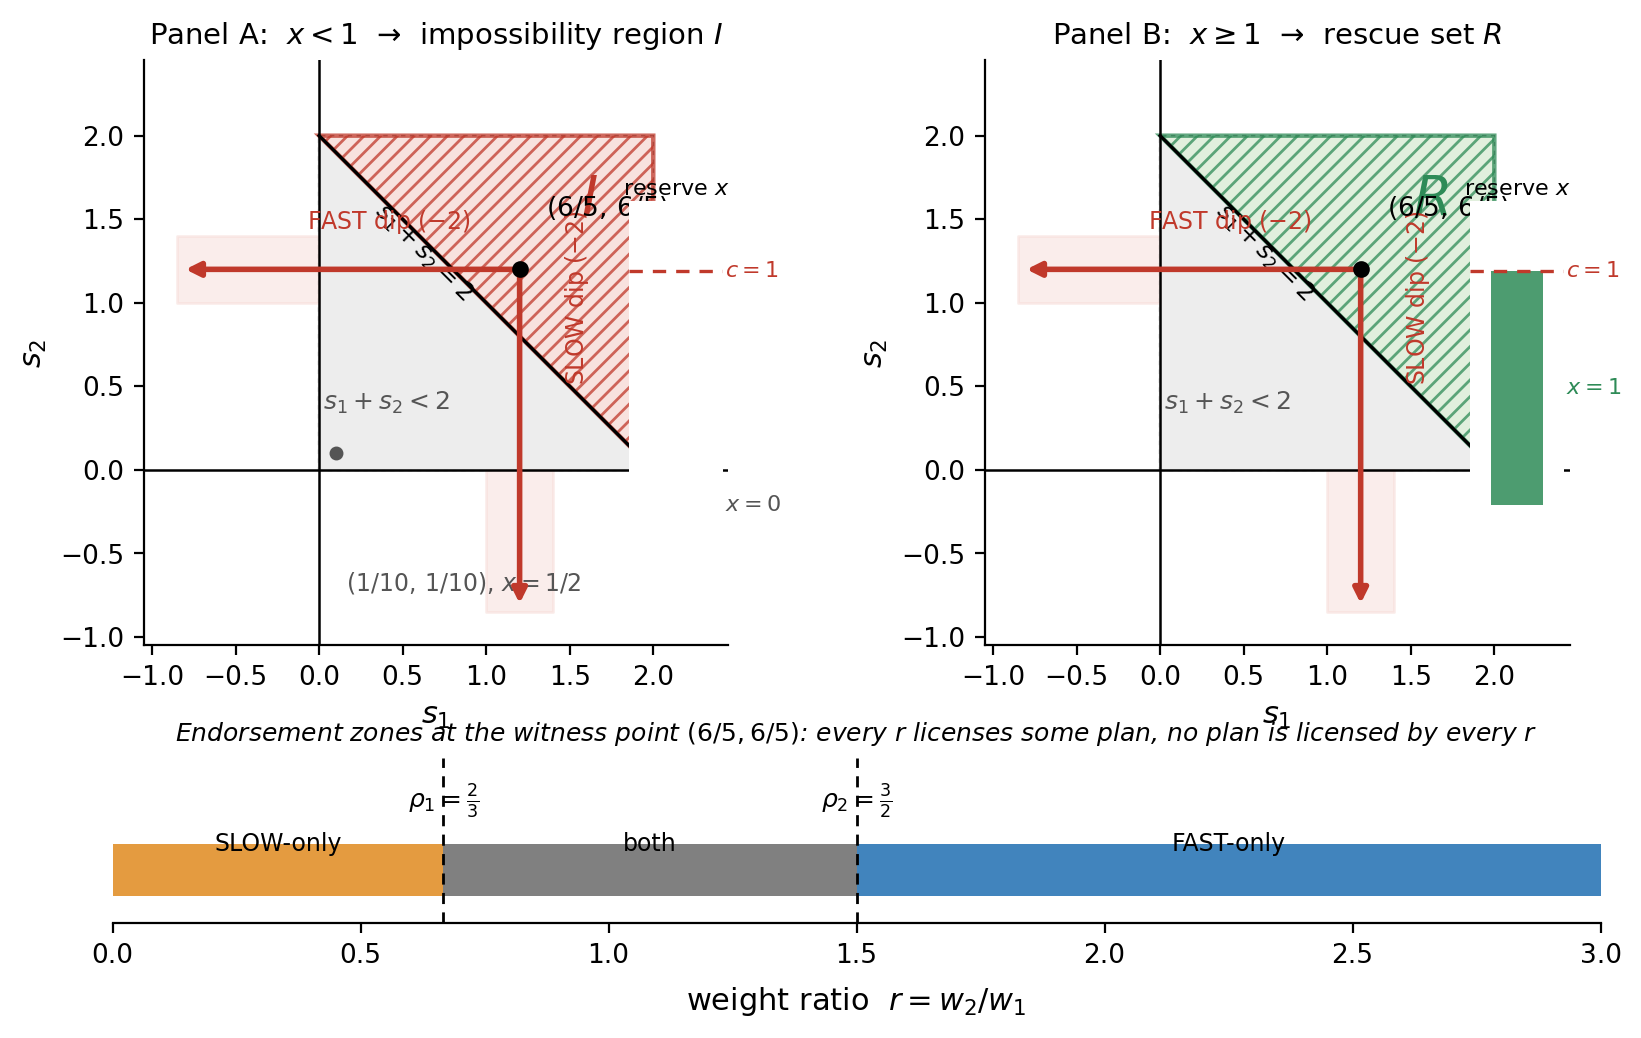
\includegraphics[width=\linewidth]{figs_p1/fig1_witness_v38.png}
\caption{The discrepancy triangle \(\mathcal{Q} = \{ s_1 < 2,\; s_2 < 2,\; s_1 + s_2 \ge 2 \}\) in the floor plane (boundary conventions as in Section 4.6). \textbf{Panel A (\(x < 1\)):} \(\mathcal{Q}\) is the impossibility region \(I = \mathrm{FP}_{\mathrm{agg}}\) --- every weighting licenses a plan, no plan satisfies the floors --- and the worst-case dip arrows show FAST (\(s_1 \to s_1 - 2\)) and SLOW (\(s_2 \to s_2 - 2\)) crossing the zero floors from the witness point \((6/5, 6/5)\). \textbf{Panel B (\(x \ge 1\)):} the same triangle is the rescue set \(R\), served by STAGED. Below the diagonal \(s_1 + s_2 = 2\), both assessments reject when \(x < 1\) and both accept when \(x \ge 1\). The reserve bars show the bridge stock \(x\) against the rescue cost \(c = 1\) (Panel A: \(x = 0\); Panel B: \(x = 1\)). The bottom strip records the endorsement zones at the witness point: SLOW-only for \(r < \rho_1 = \tfrac23\), both for \(\rho_1 \le r \le \rho_2 = \tfrac32\), FAST-only for \(r > \rho_2\).}
\end{figure}

\begin{figure}[htbp]
\centering
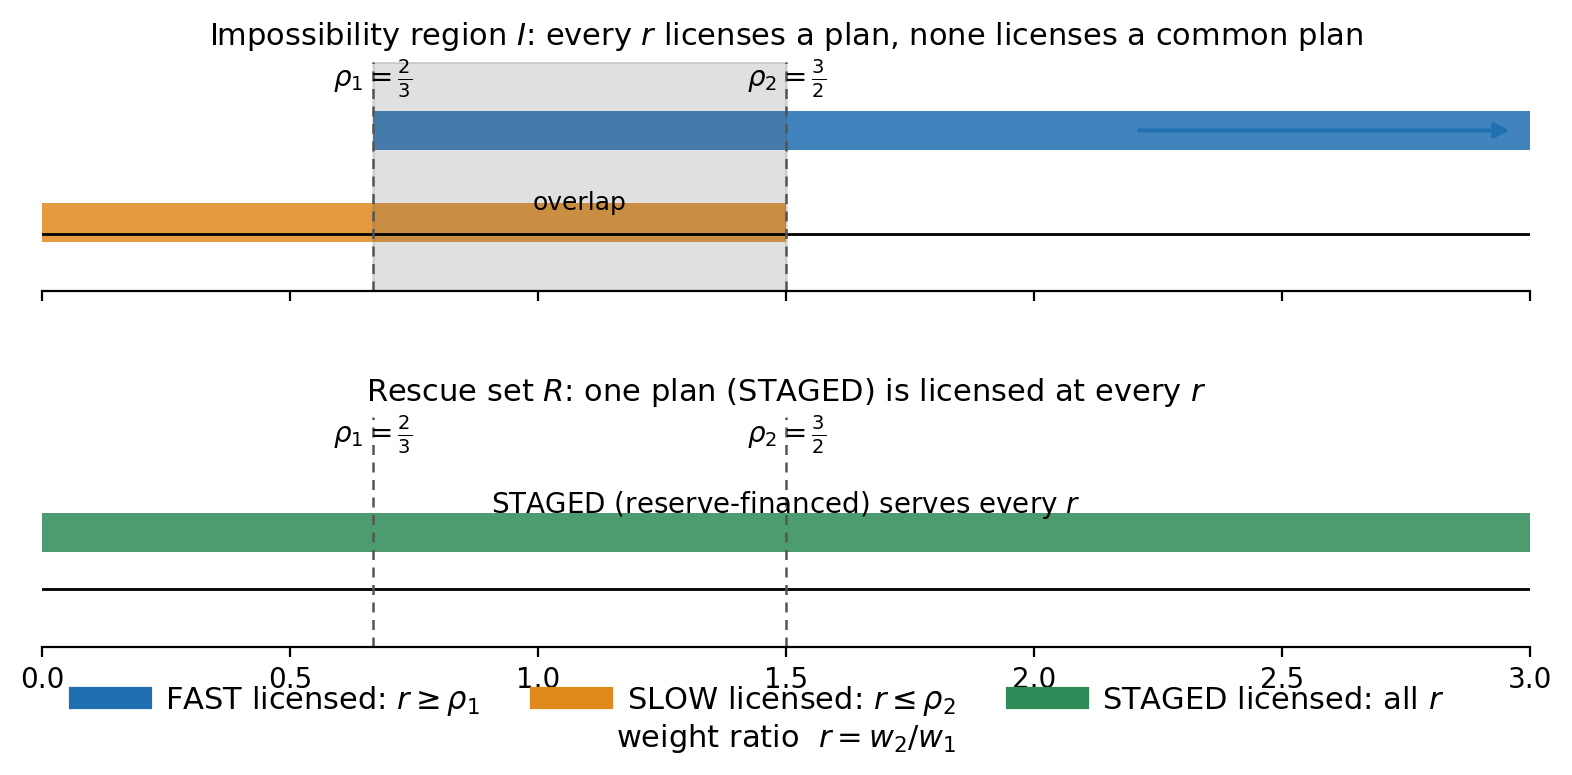
\includegraphics[width=0.98\linewidth]{figs_p1/fig2_weight_intervals_v35.png}
\caption{Weight-interval view at the witness point \((x, s_1, s_2) = (\tfrac12, \tfrac65, \tfrac65)\). FAST is licensed exactly for \(r \ge \rho_1 = \tfrac23\) and SLOW exactly for \(r \le \rho_2 = \tfrac32\). The two intervals together cover every weight ratio \(r \ge 0\), but neither covers it alone: every weight licenses a plan, no plan is licensed by every weight. On the rescue set, STAGED supplies the full interval and closes the gap.}
\end{figure}

\begin{figure}[htbp]
\centering
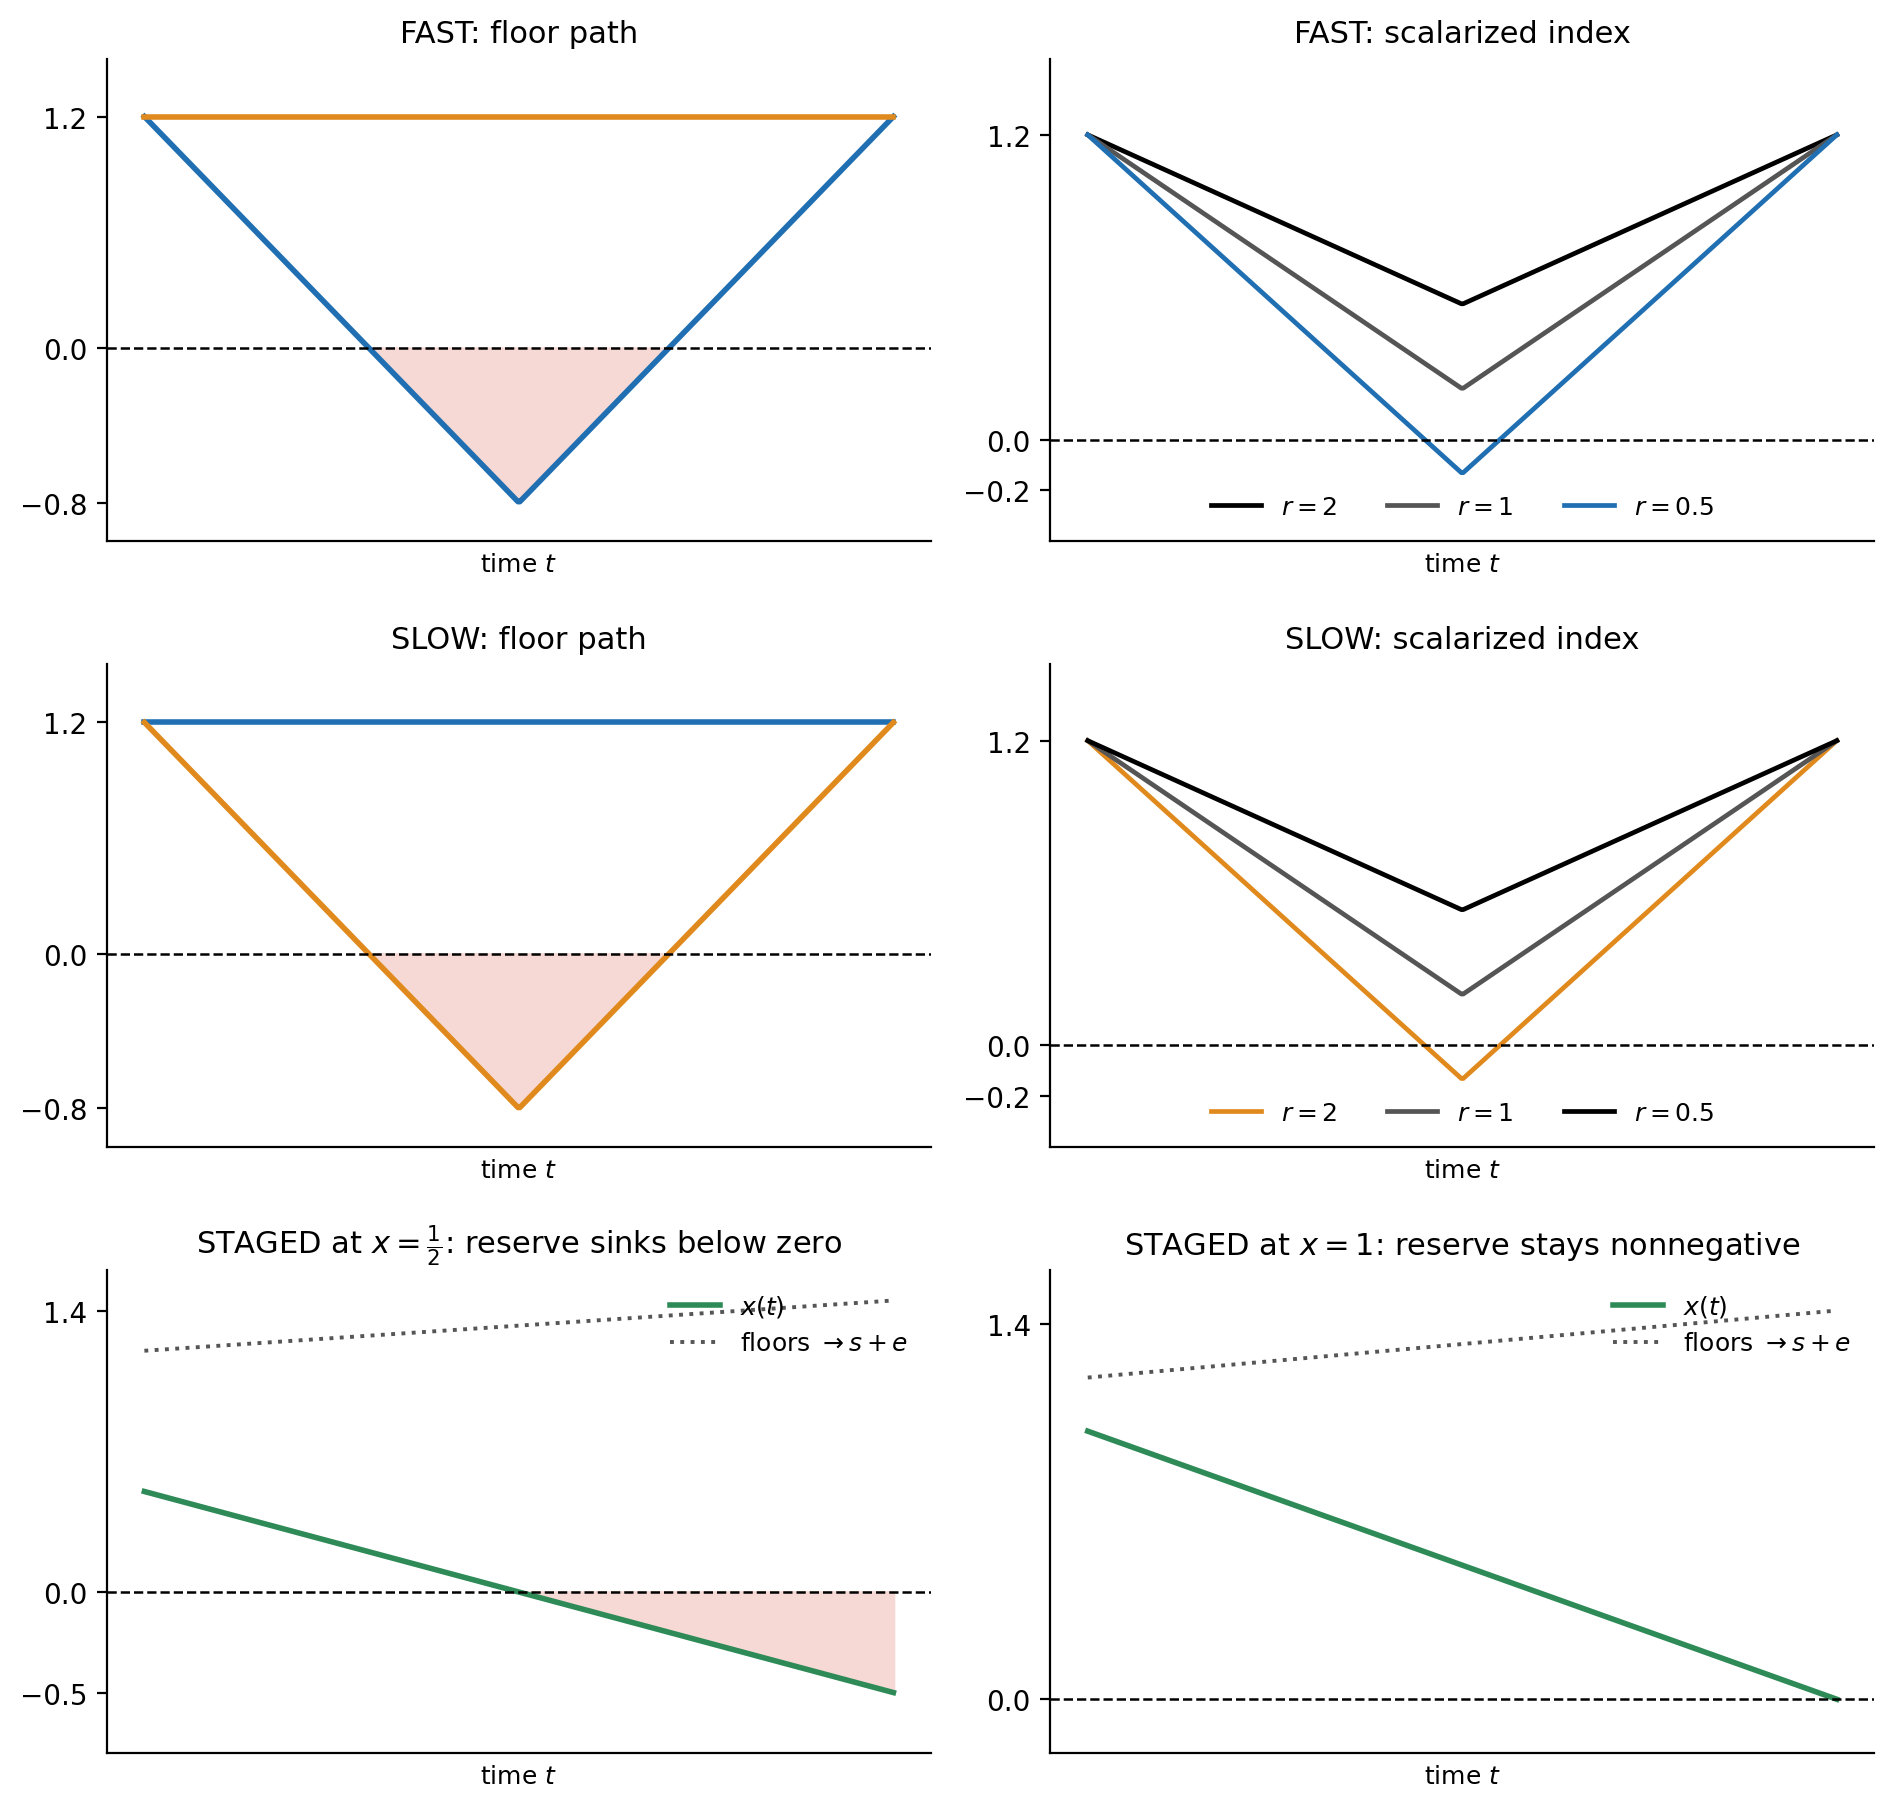
\includegraphics[width=0.98\linewidth]{figs_p1/fig3_path_view_v31.png}
\caption{Path view at the witness point. Rows: FAST, SLOW, STAGED under the worst-case disturbance; solid curves are the constrained paths, the dashed line the zero floor, and the colored curves the scalarized index for \(r \in \{2, 1, \tfrac12\}\). Under FAST (top row) the index stays nonnegative for \(r = 2\) and \(r = 1\) while \(s_1\) breaches its floor; under SLOW (middle row) the mirror holds. The only plan that protects both floors (bottom row, STAGED) consumes the reserve linearly: it is infeasible at \(x = \tfrac12\) and feasible at \(x = 1\), which is what separates the impossibility region from the rescue set.}
\end{figure}

\subsection{Propagation under hold-prefix
extension}\label{propagation-under-hold-prefix-extension}

This subsection asks whether the one-interval separation survives when
the horizon is lengthened by prepending hold intervals. Two results
delimit the answer. Remark 6 establishes persistence under a precisely
specified hold-prefix extension; Theorem 7 exhibits a two-stage datum on
which the gap is erased, showing the persistence claim is
architecture-conditional.

\textbf{Remark 6 (propagation).} \emph{Extend the witness datum to
\(m \ge 2\) review intervals by prepending hold intervals (sole action
HOLD: constant tube \(\{z\}\), successor \(\{z\}\), safe set \(S_0\);
the final interval carries the witness). Assume:}

\begin{itemize}
\tightlist
\item
  \emph{(H1) HOLD is available at every prefix state;}
\item
  \emph{(H2) the hold tube is exactly \(\{z\}\);}
\item
  \emph{(H3) the prefix safe sets contain the witness states;}
\item
  \emph{(H4) terminal and successor architecture labels are unchanged;}
\item
  \emph{(H5) no additional reset or disturbance branches are
  introduced.}
\end{itemize}

\emph{Then:}

\emph{(i) Hierarchy.} \emph{For every stage \(j\),}
\[\mathcal{V}^{\mathrm{typ}}_j \;\subseteq\; \bigcap_{w \in W_+} \mathcal{V}^{w}_j \;\subseteq\; \mathcal{V}^{\mathrm{phys}}_j.\]
\emph{This inclusion holds for every multi-interval typed exact-tube
datum; it is constraint monotonicity under backward induction.}

\emph{(ii) Persistence of strictness.} \emph{The stage-0 accepted
regions are the witness regions pulled back through the holds, so both
strictness witnesses of Theorem 5 persist under this hold-prefix
extension.}

\emph{(iii)} \emph{The displayed separation is not an artifact of the
one-interval framing for the constructed hold-prefixed datum. Strictness
for arbitrary multi-stage systems does not follow without a separate
persistence theorem: a later stage can erase the gap if every
aggregate-feasible state has a common typed-safe continuation, if the
weak and typed terminal sets coincide on the reachable subset, or if
actions couple across stages.}

\emph{Proof.} See Appendix B.\textbf{Theorem 7 (erasure witness).} \emph{The propagation claim of
Remark 6 is architecture-conditional: there is a two-interval datum
whose single-interval truncation exhibits the acceptance gap and whose
two-stage extension erases it, through the terminal-coincidence
mechanism of Remark 6(iii).}

\emph{Proof.} See Appendix B.The witness datum of Section 4.5 is not subject to this erasure. Its gap is
tube-driven: on \(I\) every member of the four-action menu violates the
stage-1 path constraint \(S_0\) itself (the two dips and the bridge
deficit of Theorem 5(7)), and a later stage cannot repair a violated
tube --- the stage-1 constraint is local to stage 1. Remark 6's safe
direction is secured by exactly the assumptions the erasure datum
violates (unchanged terminal architecture, no new branches). The two
results together delimit the persistence claim: hold-prefix extension
preserves the separation, arbitrary multi-stage extension does not, and
the erasure mechanisms of Remark 6(iii) are realizable.

\subsection{Machine verification}\label{machine-verification}

Proposition 3, Proposition 4, Theorem 5, Remark 6, and Theorems 7--8
are proved in Appendices A--C. An accompanying software artifact (deterministic exact-integer arithmetic; no floating point, tolerances, or randomness) checks the finite rational instance of Proposition 3, Proposition 4, Theorem 5, and Remark 6: the action classifications, the region identities, and the accepted-set identities on a \(31^3 = 29{,}791\)-state grid over \((x, s_1, s_2)\), with a finite verification set containing the critical weight ratios \(\rho_1, \rho_2\) and their midpoint for every enumerated grid state. All 25 checks pass and re-execution reproduces them exactly; they are enumerated in the Supplementary Material (S8).
\noindent\begin{tabular}{@{}
  >{\raggedright\arraybackslash}p{(\columnwidth - 4\tabcolsep) * \real{0.3333}}
  >{\raggedright\arraybackslash}p{(\columnwidth - 4\tabcolsep) * \real{0.3333}}
  >{\raggedright\arraybackslash}p{(\columnwidth - 4\tabcolsep) * \real{0.3333}}@{}}
\toprule\noalign{}
\begin{minipage}[b]{\linewidth}\raggedright
Claim layer
\end{minipage} & \begin{minipage}[b]{\linewidth}\raggedright
What is established
\end{minipage} & \begin{minipage}[b]{\linewidth}\raggedright
By what
\end{minipage} \\
\midrule\noalign{}
Continuum statements & Exact identities and inequalities on the witness datum & Appendices A--C \\
Finite rational instance & Classifications on the enumerated grid & Deterministic computation \\
Empirical claims & None in this article & --- \\
\bottomrule\noalign{}
\end{tabular}

The finite grid does not by itself prove the continuum identities; it
validates the symbolic classification on the enumerated instance.

\subsection{Menu convexification: the blend
family}\label{menu-convexification-the-blend-family}

The action space is the finite menu \{FAST, SLOW, STAGED,
NO-SWITCH\} of deterministic actions; fractional or alternating policies
are not members of it. The convexification instrument is the blend
family: for each \(\delta \in (0,1)\), the action BLEND\(_\delta\) is
the \emph{convexified action} obtained by fractional allocation of the
primitive control flows,
\(u_\delta = \delta\, u_{\mathrm{FAST}} + (1-\delta)\, u_{\mathrm{SLOW}}\);
by linearity of the flow map its worst-case tube is the pointwise convex
combination of the two primitive worst-case tubes and its successor the
convex combination of the two successors. This is menu convexification
at the level of control inputs --- an explicit model assumption, not the
time-sharing of discrete actions in alternation.

\textbf{Theorem 8 (blend collapse).} \emph{On the witness datum of
Section 4.5, over initial states \(X_0\):}

\emph{(i)} \emph{BLEND\(_\delta\) is typed-admissible at \(z\) exactly
when}
\[\delta \in \left[\,1 - \frac{s_2}{2},\; \frac{s_1}{2}\,\right],\]
\emph{an interval nonempty exactly when \(s_1 + s_2 \ge 2\) (a singleton
at equality), independent of \(x \ge 0\) and of the weight.}

\emph{(ii)} \emph{The typed acceptance set of the menu augmented by the
blend family is exactly the compensatory region:}
\[\mathcal{V}_{\mathrm{typ}}^{\mathrm{blend}} \;=\; \{ x \ge 1 \} \cup \{ s_1 + s_2 \ge 2 \} \;=\; \mathcal{V}_{\mathrm{weak}}.\]
\emph{Convexification of the menu collapses the acceptance gap:
\(\mathrm{FP}_{\mathrm{agg}}\) vanishes under the augmented menu, and
the blend family reaches exactly the compensatory region and nothing
beyond --- on
\(\mathcal{V}_{\mathrm{phys}} \setminus \mathcal{V}_{\mathrm{weak}}\) no
blend is typed-admissible.}

\emph{(iii)} \emph{The admissible window depends on the state through
\((s_1, s_2)\) alone: a single \(\delta\) serves every weight
\(w \in W_+\). On the impossibility region the blend is therefore the
common action that no member of the finite menu supplies --- the
acceptance gap is a property of the deterministic menu, not of the
doctrines.}

\emph{Proof.} See Appendix B.\emph{Remark.} The collapse is exact and weight-independent: a single
convexified plan serves every assessor on \(I\), where the per-weight
plans of Theorem 5(6) necessarily differ. The nonconvexity at work is
menu geometry --- the finiteness and determinism of the action space ---
not the Pareto-frontier geometry under which weighted sums fail to reach nonconvex frontier parts (Das and Dennis, 1997); the two mechanisms are distinct. The structure is precisely that of
pure-versus-mixed strategies in the assessor--planner game (von Neumann,
1928; Sion, 1958): with the planner picking an action, the assessor a
weight, and the payoff the worst-case aggregate, common-plan acceptance
is the pure-strategy value and per-weight acceptance the mixed value,
the gap being the pure-strategy duality gap that the convex (mixed)
extension closes. The two-player reach/avoid formulation of such games is the discriminating kernel of Cardaliaguet (1996), with numerical treatment in Cardaliaguet, Quincampoix, and Saint-Pierre (1999). This is also the here-and-now versus wait-and-see
separation of adjustable robust optimization (Ben-Tal et al., 2004).

\subsection{The converse: discrete time-sharing does not erase
the
gap}\label{the-converse-discrete-time-sharing-does-not-erase-the-gap}

\textbf{Proposition 9 (sequential time-sharing does not erase the gap).}
\emph{On the witness datum of Section 4.5, let a sequential time-shared
policy alternate between FAST and SLOW over the interval, so the set of
visited states is the union of the two primitive worst-case tubes. Then
such a sequential policy is typed-admissible if and only if
\(s_1 \ge 2\) and \(s_2 \ge 2\); on the impossibility region \(I\)
(where \(s_1 < 2\), \(s_2 < 2\), \(s_1 + s_2 > 2\)) no such policy is
typed-admissible, and the acceptance gap therefore survives discrete
time-sharing.}

\emph{Proof.} See Appendix B.\emph{Remark.} Together Proposition 9 and Theorem 8 delimit the notion
of mixing precisely: continuous convexification --- fractional
allocation of control flows --- closes the acceptance gap exactly at the
compensatory region \(s_1 + s_2 \ge 2\), whereas discrete time-sharing
--- alternation in time, whose visited set is the union of the action
tubes --- closes it only where the two dips are independently subsumed,
\(s_1 \ge 2\) and \(s_2 \ge 2\). On the regime \(s_1 + s_2 \ge 2\) with
\(\min(s_1, s_2) < 2\) (which contains the impossibility region) the gap survives sequential time-sharing and closes only under convexification, so the structural character of the gap is a property of
the \emph{convexity of the action space}, not of the assessment doctrine
and not of temporal sharing as such.

\begin{center}\rule{0.5\linewidth}{0.5pt}\end{center}

\section{Interpretation}\label{interpretation}

\subsection{The doctrinal reading}\label{the-doctrinal-reading}

The scalarized operators \(\{E_w\}_{w \in W_+}\) formalize \textbf{one}
compensatory assessment doctrine. The doctrine comprises: a single
aggregate index \(w \cdot s\); nonnegative scalarization weights on
capital forms; substitution across floors permitted at those weights;
and disturbances respected. We refer to this as \emph{the scalarized
aggregate doctrine as formalized here}, not as ``weak sustainability''
simpliciter. The weak-sustainability literature is broader than this
operator: it encompasses aggregate wealth, constant total capital,
nondeclining comprehensive consumption, substitutability assumptions,
discounting, shadow prices, and intertemporal investment conditions
(Neumayer, 2013; World Bank, 2011; Boos, 2015; Dasgupta and M\"aler, 2000;
Asheim, 1994). Likewise, strong sustainability is not always equivalent
to requiring every stock coordinate to remain nonnegative at every
instant. Critical-natural-capital frameworks may use thresholds, safe
operating spaces, irreversibility, resilience, or minimum-service
conditions (Ekins et al., 2003; Doyen and Gajardo, 2020). The typed
operator \(E_{\mathrm{typ}}\) is a formal idealization of the
separately-binding-floor reading, in the same sense that the scalarized
operators idealize one aggregation doctrine. The typed operator is the
coordinate-wise criterion --- each floor is required to hold separately ---
and the scalarized family is the compensatory criterion; the two vocabularies
name the same operators, with \emph{typed} denoting the framework object and
\emph{coordinate-wise} its constraint structure.

Within this precise scope, Theorem 5 reads as follows. The two
formalized doctrines can disagree on the same transition datum, with the
same robustness standard and the same action set, in the direction
compensatory-accepts / noncompensatory-rejects, on a relatively open
region. The disagreement is not an artifact of one bad weight: every
weight accepts, each licensing a different physical transition. The
plans are genuinely different transitions (FAST and SLOW violate
different floors at different times), which is the dynamic formalization
of substitution across floors. By Proposition 3(ii), the precise seat of
the disagreement is the noncommutativity of ``choose an action'' with
``for all weights.''

At the static level the full-cone aggregate is lossless (Remark 2), so the compensatory doctrine's limitation is not the existence of an aggregate index but the \emph{policy dependence} of the aggregate-feasible transition: the index certifies a set of transitions, none of which the noncompensatory assessment accepts. The two
quantifier orders also carry an information reading.
\(\exists a\, \forall w\) is a commitment made before the weight is
known --- the strong doctrine's robustness demand --- while
\(\forall w\, \exists a_w\) lets the action be chosen after the weight
is observed. On the witness, the acceptance gap between the two orders
measures the value of information about the assessment weight. Theorem 8 qualifies this reading: a single convexified blend serves every weight on the impossibility region, so the value of information reflects the finite deterministic menu rather than the weight information itself. Proposition 9 sharpens the point: the value of information is removed by convexifying the action space, not by sharing actions in time --- under discrete time-sharing the gap (and
hence the value of information about the weight) survives on the
impossibility region.

Throughout, we use ``nonnegative scalarization weights'' for elements of
\(W_+\) and reserve the word ``prices'' for the interpretive discussion.
Actual prices may be strictly positive, endogenous,
dynamically determined, state-dependent, or dimensionally heterogeneous,
and the theorems require none of those properties. The operators are
linear scalarizations with weights fixed over the review interval.
Nonlinear aggregate indices --- CES-type substitutability or endogenous,
state-dependent weighting of the kind that diverges near zero-stock
boundaries --- are different assessment operators, and the theorems
claim nothing for them.

\subsection{Positioning against established
theory}\label{positioning-against-established-theory}

The backward recursion of Section 3 is
a typed instance of established robust-predecessor, reach-avoid,
capture-basin, and hybrid-reachability constructions (Aubin, 1991;
Aubin, Bayen, and Saint-Pierre, 2011; Saint-Pierre, 1994; Lygeros,
Tomlin, and Sastry, 1999); the fixed-point and algebraic character of these objects is developed in Aubin and Catt\'e (2002). Proposition 3(i) is constraint-set
monotonicity of viability kernels and reachability sets (Aubin, 1991;
Frankowska, 1989). The foundation statement that values may be only
weakly comparable --- and that this incommensurability is constitutive
of ecological economics --- is due to Martinez-Alier, Munda, and O'Neill
(1998). Our operators give one formal model of the distinction that
paper draws between strong and weak commensurability. The
characterization of which sustainability criteria admit indicator
representations, and the role of maximin and MSY-type reasoning in
making strong sustainability operational, are developed in Martinet
(2011), Cairns and Martinet (2014), and Doyen and Gajardo (2020). The
latter in particular shows that the multicriteria maximin value is the
solution of a static Pareto problem over the viability kernel, which is
the strongest formal statement in the literature of the position ---
strong sustainability as constraint viability rather than optimality ---
that the typed operator formalizes here.

Static scalarization
limitations are established: weighted sums cannot reach nonconvex parts
of Pareto fronts (Das and Dennis, 1997), a mechanism of frontier
geometry under a single optimization, different from the
action-quantifier mechanism of this paper. Compensability analysis is
established in multi-criteria decision analysis, including the explicit
mapping of compensatory aggregation to weak sustainability and
outranking methods to strong sustainability (Cinelli, Coles, and Kirwan,
2014; Sch\"ar, Pohl, and Geldermann, 2025). Scalarization-dependent
optimal policies are a staple of multi-objective optimization.

Against this background, the finite-menu characterization of
Section 4.4 is the general form, of which the witness separation
(Theorem 5) and the blend collapse (Theorem 8) are the instances.

To our knowledge, no explicit exact-tube witness for this dynamic
separation in a compensatory/noncompensatory assessment setting is
reported in the literature. We do not assert priority over the
elementary quantifier fact
\(\exists a\, \forall w \neq \forall w\, \exists a_w\), which is
standard. Whether an equivalent dynamic separation appears in adjacent
literatures (multi-objective robust control, viability theory,
multi-criteria decision analysis) is not established either way.

\subsection{Scope delimitations}\label{scope-delimitations}

\begin{itemize}
\tightlist
\item
  \textbf{No separation on every datum.} Where a single action is safe
  for all weights, the assessments coincide. The theorem is an existence
  separation with an open region, plus the always-valid hierarchy and
  localization.
\item
  \textbf{No infinite-horizon, stochastic, partial-observation, or
  endogenous-event extension.} All statements are for finite-horizon exact-tube data with specified disturbance sets.
\item
  \textbf{No claim that the full nonnegative cone is the only reasonable
  weight family.} Proposition 4 shows that restricting the family
  enlarges the compensatory accepted set, so the full cone is the strictest compensatory reading, and the separation persists a fortiori for restricted families.
\item
  \textbf{No welfare claim about prices.} The weights model an
  assessment doctrine, not a normative endorsement.
\item
  \textbf{No empirical transfer.} The theorems concern assessment operators on a specified datum and imply no empirical claim about any resource system.
\item
  \textbf{No claim that \(\mathcal{V}_{\mathrm{weak}}\) is the
  genuine-savings or inclusive-wealth criterion.} The operator is the
  strictest compensatory reading (every weight, each licensing an
  action). The genuine-savings literature's criterion is a different
  object, and the witness's reserve stock is excluded from the weighted aggregate by construction (Section 4.5), not by consequence of aggregation. If the reserve entered the aggregate with positive weight, the gap could shrink or disappear; the separation isolates the case in which the aggregate measures the service floors while the reserve is a separate policy instrument.
\item
  \textbf{No absolute impossibility.} The impossibility region is a negative certificate relative to the specified four-action menu; with a larger menu it can shrink or vanish (see the completeness requirement in Section 5.5).
\item
  \textbf{No universal doctrinal ranking.} The inclusion
  \(\mathcal{V}_{\mathrm{typ}} \subseteq \mathcal{V}_{\mathrm{weak}} \subseteq \mathcal{V}_{\mathrm{phys}}\)
  is a theorem about the defined operators under common action and
  disturbance classes, common safe-set inclusion, common horizon, common
  tube semantics, and common terminal condition. It does not establish a
  universal ranking of endpoint, weak, and strong sustainability
  doctrines.
\item
  \textbf{No separation under coupled all-floor shocks.} The witness
  disturbance convention is action-indexed (Section 4.5): each action's
  worst case is its own characteristic dip. A datum whose disturbance
  class couples simultaneous dips across all floors of every action
  degenerates the per-weight licensing structure --- the principal
  actions fail together and the compensatory/noncompensatory divergence
  collapses into universal rejection. The separation is exhibited for, and scoped to, the specified action-indexed class: the witness datum assumes separable transition risks, with each plan exposing a different floor to its own adverse disturbance. That the coupled regime is not a remote possibility is indicated by evidence that planetary-boundary processes interact and amplify one another (Lade et al., 2020).
\item
  \textbf{Convexification of the menu.} Fractional action policies are
  not members of the action space, and every stated separation is scoped
  to the finite deterministic menu. Theorem 8 resolves the convexification question: the blend family collapses the typed acceptance set exactly onto the compensatory
  region, so the separation is a property of the deterministic menu, not
  of the doctrines --- menu geometry, distinct from the Pareto-frontier
  geometry of scalarization limits (Das and Dennis, 1997). The
  associated delimitation (Proposition 9) is that discrete time-sharing
  does not effect the same collapse: on the impossibility region the gap
  survives alternation in time, so the structural character of the separation is due to the convexity of the action space, not to temporal sharing.
\end{itemize}

\subsection{Policy implications}\label{policy-implications}

The separation theorem has four implications.

\textbf{First.} Aggregate indices alone cannot certify noncompensatory
transition safety under the present assessment semantics. A scalarized
assessment can certify its own criterion --- aggregate feasibility; what
it cannot certify is typed safety unless an additional bridge theorem is
supplied. This follows from Theorem 5: the compensatory accepted set
strictly contains the noncompensatory accepted set, and the excess
region is where the two criteria diverge.

\textbf{Second.} When the typed recursion identifies an admissible
rescue action whose feasibility is controlled by a resource margin,
investment in that margin is a candidate remedy; reweighting alone cannot substitute for it on the witness datum (Section 5.5). This applies where a resource-controlled rescue action exists; it is not a universal policy claim.

\textbf{Third.} Per-floor reporting alongside aggregate reporting is
necessary for detecting this class of discrepancy. It is not universally
necessary for every sustainability judgement; but where the question is
whether a transition respects separately-binding floors, an aggregate
index alone cannot distinguish the rescue region from the impossibility region. The same separately-checked-floor logic underlies the safe-and-just-space (``doughnut'') literature, which evaluates social thresholds and biophysical ceilings independently, without cross-compensation, and reports that no country satisfies all floors within all ceilings (O'Neill et al., 2018; Fanning et al., 2022). A minimum report for such an assessment should include: (1)
typed floors and their provenance; (2) aggregate weights or the weight
family; (3) policy quantifiers; (4) the disturbance set; (5) the
observation and implementation model; (6) exact versus conservative tube
status; (7) terminal maintainability; (8) action-exhaustion status; (9)
uncertainty and approximation bounds; (10) normative premises.

\textbf{Fourth.} Reporting regimes that evaluate endpoints only, as in audited annual snapshots, evaluate only the weakest operator of the chain of Section 3.1. Under those semantics they license transitions that violate typed floors mid-interval without detection (on the witness datum, FAST is typed-endpoint-admissible at every state of \(X_0\) but typed-tube-admissible only for \(s_1 \ge 2\), by inspection of the action table in Section 4.5); the per-floor reporting of the third implication detects the discrepancy. No empirical claim about any particular reporting regime is made here.

The instruments that act on the acceptance gap close it in sharply
different ways; Table~\ref{tab:instruments} records them.

\begin{table}[htbp]
\centering
\small
\begin{tabular}{@{}p{0.22\linewidth}p{0.36\linewidth}p{0.34\linewidth}@{}}
\toprule
Instrument & Mathematical operation & Effect on the gap \\
\midrule
Reweighting & change the weight \(w\) & does not close the gap \\
Restricting the weight family & replace \(W_+\) by \(W \subset W_+\) & enlarges per-weight acceptance; leaves the common-plan problem unless one plan works for all retained weights \\
Reserve augmentation & add STAGED when \(x + \kappa \ge 1\) & closes the gap for states where only the reserve constraint binds \\
Menu convexification & replace \(\mathcal{D}\) by \(\operatorname{conv}(\mathcal{D})\) (the blend family) & closes the gap exactly on the scalarized feasible region \\
Discrete time-sharing & union of the primitive tubes & generally does not close the gap; closes only where both dips are separately survivable \\
\bottomrule
\end{tabular}
\caption{Policy instruments acting on the acceptance gap.}
\label{tab:instruments}
\end{table}

\subsection{Rescue as action synthesis, and data
requirements}\label{rescue-as-action-synthesis-and-data-requirements}

\textbf{Rescue as action synthesis.} Rescue is an operation on the impossibility region. Define a resource-augmentation map
\[\mathsf{Aug}_\kappa : (x, s, \mathcal{A}) \mapsto (x + \kappa,\; s,\; \mathcal{A} \cup \{\mathrm{STAGED}_\kappa\})\]
and the minimal rescue threshold
\[\kappa^* = \inf\{\, \kappa : \exists a \in \mathcal{A}_\kappa,\; a \in E_{\mathrm{typ}}(z) \,\},\]
where \(\mathcal{A}_\kappa\) denotes the augmented menu. \textbf{Proposition (rescue threshold).} \emph{On the witness datum, for every \(z \in X_0\),}
\[\kappa^*(z) = (1 - x)_+ \cdot \mathbf{1}[\,x < 1,\; s_1 < 2,\; s_2 < 2\,] = (1 - x) \cdot \mathbf{1}[\,z \notin \mathcal{V}_{\mathrm{typ}}\,].\]
\emph{Proof.} See Appendix C.On the impossibility region \(I\), \(\kappa^*(z) = 1 - x > 0\); on the rescue set \(R\), and on all of \(\mathcal{V}_{\mathrm{typ}}\), \(\kappa^*(z) = 0\), matching the observation that states of \(R\) need no augmentation. Because \(\mathrm{STAGED}_\kappa\) is admissible exactly when \(x + \kappa \ge 1\), independently of the floors, the resource route admits every state with \(x < 1\) --- including states outside \(\mathcal{V}_{\mathrm{weak}}\), such as \((\tfrac12, \tfrac1{10}, \tfrac1{10})\) --- at cost \(1 - x\); the impossibility region is exactly the set on which the four-action menu fails yet resource augmentation succeeds at finite cost. The increment converts an impossibility-region state into a typed-transformable one.

\textbf{Remark (error-bound modulus).} Along the resource route the minimal increment is the affine function \(f(z) = (1 - x)_+\), whose error-bound modulus (Fabian et al., 2010) is identically \(1\) on \(\{x < 1\}\); the rescue threshold \(\kappa^*\) therefore coincides with the error-bound modulus along this route. The coincidence reflects the linearity of the route. On data with nonlinear resource dynamics the two quantities diverge, and the error-bound modulus governs only the scaling of distance-to-feasibility under unstructured perturbation, a regime outside the present scope (Section 6.2).

\textbf{Data requirements for empirical application.} The theorem is a
result about assessment operators on a specified datum. Empirical
application requires, in addition to the typed floors, disturbance set,
action set, tube model, and destination maintainability witness of
Section 4.5, five further specifications: the completeness status of the
action set (whether \(\mathcal{A}\) is exhaustive or merely a listed
menu), calibration and identifiability data, policy and authority data,
the threshold-uncertainty semantics, and the destination
maintainability status. The itemized requirements are given in the
Supplementary Material (S9).

\begin{center}\rule{0.5\linewidth}{0.5pt}\end{center}

\section{Discussion}\label{discussion}

\subsection{Negative certificates}\label{negative-certificates}

A negative certificate --- a rejection with an exhibited violated constraint for each action, exhausting the action set --- is a complete verdict, not an inconclusive one. Theorem 5(7) is an instance: four actions, four exhibited violations, certifying impossibility on \(I\) together with the resource threshold of Section 5.5 and the per-weight licensing thresholds of Theorem 5(6). Related scored forecast-evaluation studies apply assessment discipline of the same kind to the Northern cod and Edwards Aquifer systems (Abaee, 2026, \emph{Does a Surplus-Production Ladder Improve Forecasts of Northern Cod?}; Abaee, 2026, \emph{Does a One-Pool Water-Balance Model Improve Forecasts of Edwards Aquifer Head?}); the cited studies are referenced for related work only.

\subsection{Limitations}\label{limitations}

\begin{enumerate}
\def\labelenumi{(\roman{enumi})}
\tightlist
\item
  The separation theorem is an existence result with an open region; it does not imply the gap is large in any given application, and where the assessments coincide it yields nothing.
\item
  Novelty statements reflect bounded literature search (Section 5.2).
\item
  The operators cover finite horizons with exact tubes and specified disturbance sets; infinite horizons, partial observation, stochastic chance constraints, and endogenous event times are not treated.
\item
  The finite-menu theorem of Section 4.4 governs plans whose admissibility is characterized by a required-margin vector; plans outside that class (reserve-financed plans, destination-failing plans) are handled separately, and the geometric form of the gap is established within the margin class.
\item
  If a convexified (blended) plan is physically and institutionally available, the gap disappears by Theorem 8; the separation is therefore a statement about certification relative to the available plan menu, not a claim that the gap is unavoidable in every institution.
\item
  No empirical claims are made.
\item
  The governance, intergenerational, and composition extensions are stated at partial status in the Supplementary Material and are not used in the proofs.
\item
  Computational tractability: on a finite explicit state--action--disturbance graph with constant-time predicate evaluation, the backward recursion is polynomial in the graph size and horizon. For continuous, hybrid, or belief-state models, the graph itself may be exponentially large, infinite, or only approximately representable; exact-tube inclusion may be computationally hard or undecidable; and grid cardinality grows as \(N_{\mathrm{grid}} = \prod_{i=1}^n N_i\) --- exponentially in dimension when floors are coordinates. The witness is tractable because its datum is small, finite, and rational.
\end{enumerate}

\begin{center}\rule{0.5\linewidth}{0.5pt}\end{center}

\section{Conclusions}\label{conclusions}

Scalarized and coordinate-wise feasibility criteria are usually compared
as doctrines --- as different normative stances on substitutability, of
which the weak- and strong-sustainability traditions are the canonical
instances. This paper shows that the divergence between the two criteria
as formalized here --- the scalarized-aggregate and typed
operators of Section 3.1 on a common action menu and disturbance class
--- survives translation into assessment mechanics, at the level of a
theorem about those operators. The theorem establishes no ranking of doctrines: Section 5.1 delimits the formalizations, and by Theorem 8 the structural character of the separation is a property of the finite deterministic menu, not of either tradition (Sections 4.10--4.11). On a typed transition datum under exact-tube semantics, the
compensatory reading (per-weight acceptance) and the noncompensatory
reading (common-plan acceptance) are related by a quantifier commutation
that can fail on an open region of state space. Where it fails, every
scalarization weight certifies a transition, but no single transition is
certified by all weights, and the certified set splits into states
rescuable by a resource-controlled action and states that are impossible
under every weight. The mechanism is not scalarization blindness --- at
fixed trajectories the full-cone aggregate is lossless --- but the
policy dependence of the aggregate-feasible transition. The
finite-menu theorem of Section 4.4 states the underlying mechanism in
full generality: for any finite menu, the acceptance gap is the part of
the convex hull of the required margins that no single plan dominates,
so the witness of Section 4.5 is an instance of a geometric fact rather
than an isolated construction.

For the construction of composite sustainability indices, the theorem
has a concrete consequence. An index can be sound at the level of
accounting and still over-certify at the level of assessment, because
certification is a quantifier statement about transitions, not a
property of a number. Where separately-binding floors matter, per-floor
reporting is not a presentation preference but a detection requirement:
the aggregate alone cannot distinguish the rescue region from the
impossibility region. The bridge a composite index needs --- some single
transition that serves every admissible weight, i.e.~membership in
\(\mathcal{V}_{\mathrm{typ}}\) --- is exactly what the frameworks'
reporting conventions should be asked to exhibit. Theorem 8 qualifies this requirement: such a single transition is not, in general, a member of the specified deterministic menu but a convexified action, so the relevant question for a reporting convention is whether its action set admits the required menu convexification --- and Proposition 9 shows that temporal alternation alone does not provide it.

\begin{center}\rule{0.5\linewidth}{0.5pt}\end{center}


\appendix

\section{Proofs of the general results}

\textbf{Proof of Remark 1 (Section 4.1).}\ If \(a \in \bigcap_\lambda E_\lambda(z)\), then each
\(E_\lambda(z)\) is nonempty, so \(z\) lies in the right-hand set. The
inclusion fails at \(z\) precisely when each \(E_\lambda(z)\) is
nonempty but \(\bigcap_\lambda E_\lambda(z) = \varnothing\), i.e.~when
no common selector exists; this is the stated equality condition. \ensuremath{\square}

\textbf{Proof of Remark 2 (Section 4.2).}\ (\(\Rightarrow\)) \(w \ge 0\), \(w \neq 0\), \(v \ge 0\)
gives \(w \cdot v = \sum_i w_i v_i \ge 0\). (\(\Leftarrow\)) If
\(v_k < 0\), take \(w = e_k \in W_+\): then \(w \cdot v = v_k < 0\). \ensuremath{\square}

\textbf{Proof of Proposition 3 (Section 4.3).}\ (i) Let \(a \in E_{\mathrm{typ}}(z)\). For every
disturbance \(d\),
\(\mathrm{Tube}(a,d) \subseteq S = S^{\mathrm{phys}} \cap \{s \ge 0\}\).
By Remark 2, every tube point satisfies \(w \cdot s \ge 0\) for every
\(w \in W_+\), and likewise every successor state lies in \(G^w\); hence
\(a \in E_w(z)\). The remaining inclusions follow from
\(S^w \subseteq S^{\mathrm{phys}}\),
\(G^w \subseteq G^{\mathrm{phys}}\), and
\(\mathrm{End}(a,d) \subseteq \mathrm{Tube}(a,d)\). (ii) The inclusion
\(\subseteq\) is part (i) intersected over \(w\). For the reverse
inclusion, let \(a \in \bigcap_{w \in W_+} E_w(z)\). For every \(d\) and
every tube point \(p \in \mathrm{Tube}(a,d)\), every \(w \in W_+\) gives
\(w \cdot s(p) \ge 0\), so by Remark 2 \(s(p) \ge 0\) componentwise;
hence \(\mathrm{Tube}(a,d) \subseteq S\). The same argument with
\(\mathrm{Succ}\) gives \(\mathrm{Succ}(a,d) \subseteq G\). Thus
\(a \in E_{\mathrm{typ}}(z)\). \ensuremath{\square}

\textbf{Proof of Proposition 4 (Section 4.4).}\ For the second inclusion: by Proposition 3(i),
\(E_w(z) \subseteq E_{\mathrm{tube,phys}}(z)\) for every \(w\), so
\(\mathcal{V}_w \subseteq \mathcal{V}_{\mathrm{phys}}\), and
intersecting over \(w \in W\) preserves the inclusion. For the first: if
\(z \in \mathcal{V}_{\mathrm{typ}}\), then by Proposition 3(ii) there
exists \(a \in \bigcap_{w \in W_+} E_w(z)\); this same \(a\) lies in
\(\bigcap_{w \in W} E_w(z)\), so \(E_w(z) \neq \varnothing\) for every
\(w \in W\), i.e.~\(z \in \mathcal{V}_W\). Monotonicity: intersecting
over a larger family can only shrink the intersection. \ensuremath{\square}

\textbf{Proof of the finite-menu theorem (Section 4.4).}\ (i) is the margin test restated. For (ii), if
\(s = d + v\) with \(d \in \operatorname{conv}(\mathcal{D})\) and \(v \ge 0\), then
for every \(w \ge 0\), \(w \cdot s \ge w \cdot d \ge \min_a w \cdot d_a\),
so the scalarized test holds. Conversely, suppose
\(s \notin \operatorname{conv}(\mathcal{D}) + \mathbb{R}^n_+\); this set is closed
and convex (a compact polytope plus a closed cone), so strict separation
gives \(w \ne 0\) with \(w \cdot s < w \cdot d + w \cdot v\) for every
\(d \in \operatorname{conv}(\mathcal{D})\) and every \(v \ge 0\). Since \(v\)
ranges over the whole cone, \(w \in \mathbb{R}^n_+ \setminus \{0\}\), and
taking \(v = 0\) gives
\(w \cdot s < \min_{d \in \operatorname{conv}(\mathcal{D})} w \cdot d =
\min_a w \cdot d_a\): the scalarized test fails. \ensuremath{\square}

\section{Proofs for the witness datum}

\textbf{Proof of Theorem 5 (Section 4.6).}\ \textbf{(1)} Typed admissibility requires the worst-case
tube in \(S_0\) and the successor in \(G\). NO-SWITCH never reaches
\(G\) (its successor retains \(q = 0\)), so it is never admissible. For
FAST, the worst-case \(s_1\)-tube is \([s_1 - 2, s_1]\), safe if and
only if \(s_1 \ge 2\); its successor \((1, x, s + e)\) lies in \(G\)
given \(x \ge 0\). Hence FAST is typed-admissible exactly when
\(s_1 \ge 2\). Symmetrically, SLOW is typed-admissible exactly when
\(s_2 \ge 2\). For STAGED, the floors grow through the interval and the
successor lies in \(G\); the binding constraint is the \(x\)-tube
\([x - 1, x]\), safe if and only if \(x \ge 1\). Therefore
\(E_{\mathrm{typ}}(z) \neq \varnothing\) exactly on
\(\{x \ge 1\} \cup \{s_1 \ge 2\} \cup \{s_2 \ge 2\}\).

\textbf{(2)} Fix \(w = (w_1, w_2) \in W_+\). NO-SWITCH misses \(G^w\)
and is never admissible. FAST is \(w\)-admissible if and only if its
worst-case aggregate value stays nonnegative:
\(w_1(s_1 - 2) + w_2 s_2 \ge 0\), i.e.~\(w_1 s_1 + w_2 s_2 \ge 2 w_1\)
(automatic when \(w_1 = 0\)). Symmetrically SLOW is \(w\)-admissible if
and only if \(w_1 s_1 + w_2 s_2 \ge 2 w_2\). STAGED is \(w\)-admissible
if and only if \(x \ge 1\) (the physical constraint within \(S^w\)),
since \(w \cdot s \ge 0\) holds automatically along its tube. Hence
\(z \in \mathcal{V}_w\) whenever \(x \ge 1\); and if \(x < 1\), then
\(z \in \mathcal{V}_w\) if and only if at least one of the two
inequalities above holds.

Suppose first \(x \ge 1\): then \(z \in \mathcal{V}_w\) for every \(w\),
so \(z \in \mathcal{V}_{\mathrm{weak}}\). Suppose \(x < 1\) and
\(s_1 \ge 2\) or \(s_2 \ge 2\): say \(s_1 \ge 2\); then FAST is
typed-admissible by (1), hence \(w\)-admissible for every \(w\), so
\(z \in \mathcal{V}_{\mathrm{weak}}\). It remains to treat \(x < 1\)
with \(s_1 < 2\) and \(s_2 < 2\). For \(w_1 > 0\), write
\(r = w_2/w_1\): FAST is \(w\)-admissible exactly when
\(s_1 + r s_2 \ge 2\), i.e.~\(r \ge (2 - s_1)/s_2 = \rho_1\) (using
\(s_2 > 0\); when \(s_2 = 0\) the condition reduces to \(s_1 \ge 2\),
which is excluded). SLOW is \(w\)-admissible exactly when
\(s_1 + r s_2 \ge 2r\), i.e.~\(r \le s_1/(2 - s_2) = \rho_2\) (using
\(s_2 < 2\)). The boundary weights are the same limiting cases: at
\(w_1 = 0\) (\(r \to \infty\)) FAST is licensed provided \(s_2 \ge 0\),
while SLOW is strictly rejected on the region \(s_2 < 2\);
symmetrically, at \(w_2 = 0\) (\(r = 0\)) SLOW is licensed provided
\(s_1 \ge 0\), while FAST is rejected on the region \(s_1 < 2\).
Therefore \(z \in \mathcal{V}_w\) for every \(w \in W_+\) if and only if
the intervals \(\{r \ge \rho_1\}\) and \(\{r \le \rho_2\}\) together
cover all of \([0, \infty]\), which holds exactly when
\(\rho_2 \ge \rho_1\). Computing,
\[\rho_2 \ge \rho_1 \iff \frac{s_1}{2 - s_2} \ge \frac{2 - s_1}{s_2} \iff s_1 s_2 \ge (2 - s_1)(2 - s_2) \iff s_1 + s_2 \ge 2,\]
with both denominators positive in the present case. Hence, in this
case, \(z \in \mathcal{V}_{\mathrm{weak}}\) if and only if
\(s_1 + s_2 \ge 2\). Assembling the three cases, and noting
\(\{s_1 \ge 2\} \cup \{s_2 \ge 2\} \subseteq \{s_1 + s_2 \ge 2\}\) under
nonnegativity,
\[\mathcal{V}_{\mathrm{weak}} = \{ x \ge 1 \} \cup \{ s_1 + s_2 \ge 2 \}.\]

\textbf{(3)} In the physical operators the only constraint is
\(x \ge 0\) (with \(q = 1\) at the destination). FAST and SLOW have
tubes within \(S^{\mathrm{phys}}\) and successors in
\(G^{\mathrm{phys}}\) for every \(z \in X_0\) (their dips affect only
\(s\), which is unconstrained physically); STAGED does so exactly for
\(x \ge 1\). Hence \(E_{\mathrm{tube,phys}}(z) \neq \varnothing\) for
every \(z \in X_0\), so \(\mathcal{V}_{\mathrm{phys}} = X_0\). For the
endpoint operator, the endpoint values of FAST and SLOW lie in
\(S^{\mathrm{phys}}\) for every \(z \in X_0\), so
\(\mathcal{V}_{\mathrm{end}} = X_0\) as well.

\textbf{(4)} By (1)--(2),
\[\mathrm{FP}_{\mathrm{agg}} = \mathcal{V}_{\mathrm{weak}} \setminus \mathcal{V}_{\mathrm{typ}}
= \big[ \{x \ge 1\} \cup \{s_1 + s_2 \ge 2\} \big] \setminus \big[ \{x \ge 1\} \cup \{s_1 \ge 2\} \cup \{s_2 \ge 2\} \big]\]
\[= \{ x < 1,\ s_1 < 2,\ s_2 < 2,\ s_1 + s_2 \ge 2 \} = I.\]
This set is nonempty
(e.g.~\((x, s_1, s_2) = (\tfrac12, \tfrac65, \tfrac65)\)), and its
relatively open interior is the stated region.

\textbf{(5)} By (4),
\(I = \mathrm{FP}_{\mathrm{agg}} = \mathcal{V}_{\mathrm{weak}} \setminus \mathcal{V}_{\mathrm{typ}} \neq \varnothing\),
so the first inclusion is strict. For the second, the point
\((\tfrac12, \tfrac1{10}, \tfrac1{10})\) satisfies \(x < 1\) and
\(s_1 + s_2 = \tfrac15 < 2\), so it lies outside
\(\mathcal{V}_{\mathrm{weak}}\) by (2), while by (3) it lies in
\(\mathcal{V}_{\mathrm{phys}}\).

\textbf{(6)} The threshold characterization was derived in the proof of
(2): with \(r = w_2 / w_1\), FAST is licensed exactly for
\(r \ge \rho_1\) and SLOW exactly for \(r \le \rho_2\), and
\(\rho_2 \ge \rho_1 \iff s_1 + s_2 \ge 2\). On \(\mathcal{Q}\) the
inequality \(s_1 + s_2 \ge 2\) holds, so the two licensing intervals
overlap and together cover all weights; strictly on the relative
interior (\(s_1 + s_2 > 2\)) both thresholds are finite and the
intervals overlap in a nondegenerate interval, with \(r > \rho_2\)
licensing FAST only and \(r < \rho_1\) licensing SLOW only. On \(I\)
(where \(x < 1\)), STAGED is inadmissible for every \(w\), so
\(E_{\mathrm{typ}}(z) = \bigcap_w E_w(z) = \varnothing\) by Proposition
3(ii): no single action serves every weight. On \(R\) (where
\(x \ge 1\)), STAGED lies in \(E_{\mathrm{typ}}(z) = \bigcap_w E_w(z)\)
and serves every weight.

\textbf{(7)} On \(R\), STAGED's tube is
\([x - 1, x] \times \{s \to s + e\}\): the \(x\)-tube stays nonnegative
because \(x \ge 1\), the floors grow, and the successor
\((1, x - 1, s + e) \in G\). On \(I\), the four exhibited violations
exhaust the action set and each violates a typed constraint: FAST's
\(s_1\)-tube reaches \(s_1 - 2 < 0\); SLOW's \(s_2\)-tube reaches
\(s_2 - 2 < 0\); STAGED's \(x\)-tube reaches \(x - 1 < 0\); NO-SWITCH's
successor misses \(G\). \ensuremath{\square}

\textbf{Proof of Remark 6 (Section 4.8).}\ (i) Backward induction on stages. Base: at the final stage
the terminal sets satisfy
\(G \subseteq G^w \subseteq G^{\mathrm{phys}}\) by Remark 2 and the
definition of the terminal sets. Step: the accepted set of a stage is
the set of states from which some action keeps the tube in the safe set
and the successor in the next-stage accepted set; applying Proposition
3(i) to the stage's action sets and the induction hypothesis to the
next-stage accepted sets preserves the three-way inclusion at the stage
level. (ii) With HOLD the unique prefix action, a prefix state is
accepted exactly when it lies in the prefix safe set and in the
next-stage accepted set; the stage-0 regions are therefore the witness
regions of Theorem 5 pulled back through the (identity) holds, and the
strictness witnesses (\(I \neq \varnothing\) and the point
\((\tfrac12, \tfrac1{10}, \tfrac1{10})\)) persist. (iii) The three
listed mechanisms are each sufficient to erase the gap in a multi-stage
setting, so no unconditional generalization is asserted. \ensuremath{\square}

\textbf{Proof of Theorem 7 (Section 4.8).}\ \emph{Datum.} Two capital forms, floors at zero, the bridge stock absent
(\(x \equiv 0\)); states are pairs \(s = (s_1, s_2)\). Stage 2 (final
interval): safe set \(S_0^{(2)} = \mathbb{R}^2\) (no path constraint),
terminal sets \(G^{(2)} = G^{w,(2)} = G = \{ s \ge 0 \}\) --- coincident
for every weight --- and a single action REPAIR with tube \(\{s\}\)
(safe trivially) and successor \((1, 1) \in G\). Stage 1: safe set
\(S_0 = \{ s \ge 0 \}\); two actions with constant tubes, safe at every
state of \(S_0\): A1 with successor \((s_1 - 1, s_2 + 1)\) and A2 with
successor \((s_1 + 1, s_2 - 1)\); the stage-1 terminal architecture is
the stage-2 accepted sets. Initial state \(z^* = (\tfrac25, \tfrac25)\).

\emph{In the two-stage datum the gap is erased.} REPAIR is
typed-admissible --- hence \(w\)-admissible for every weight --- from
every state, so
\(\mathcal{V}_{\mathrm{typ}}^{(2)} = \mathcal{V}_w^{(2)} = \mathbb{R}^2\)
for every \(w\): the stage-2 accepted sets coincide. Backward induction
then admits both A1 and A2 at \(z^*\) (safe tubes; successors in
\(\mathcal{V}_{\mathrm{typ}}^{(2)} = \mathbb{R}^2\)), so \(z^*\) is
typed-accepted at stage 0, and weak acceptance follows from typed
acceptance.

\emph{In the single-interval truncation --- the same stage-1 datum with
the final interval collapsed to its terminal sets, \(G = \{s \ge 0\}\)
and \(G^w = \{w \cdot s \ge 0\}\) --- the gap is present.} Both
successors leave \(G\) (\(s_1 - 1 = -\tfrac35 < 0\) and
\(s_2 - 1 = -\tfrac35 < 0\)), so \(z^*\) is typed-rejected. For the weak
doctrine, writing \(r = w_2 / w_1\) on the interior of the weight cone:
A1 is \(w\)-admissible exactly when \((s_1 - 1) + r (s_2 + 1) \ge 0\),
i.e.~\(r \ge \tfrac{1 - s_1}{s_2 + 1} = \tfrac37\); A2 exactly when
\((s_1 + 1) + r (s_2 - 1) \ge 0\),
i.e.~\(r \le \tfrac{s_1 + 1}{1 - s_2} = \tfrac73\); the two intervals
cover \([0, \infty]\) because \(\tfrac37 < \tfrac73\), and the boundary
weights are covered directly (\(r = 0\): A2 gives
\(w_1(s_1 + 1) \ge 0\); \(r \to \infty\): A1 gives
\(w_2(s_2 + 1) \ge 0\)). Hence \(z^* \in \mathcal{V}_{\mathrm{weak}}\)
in the truncation, and the gap
\(\mathcal{V}_{\mathrm{weak}} \setminus \mathcal{V}_{\mathrm{typ}}\)
contains \(z^*\). \ensuremath{\square}

\textbf{Proof of Theorem 8 (Section 4.10).}\ (i) FAST's worst-case tube has \(s_1\)-coordinates
\([s_1 - 2, s_1]\) and \(s_2\)-coordinate \(\{s_2\}\); SLOW's has
\(s_1\)-coordinate \(\{s_1\}\) and \(s_2\)-coordinates
\([s_2 - 2, s_2]\); both keep \(x\) nonnegative throughout (their dips
affect only \(s\)). The blended tube therefore has \(s_1\)-coordinates
\([s_1 - 2\delta, s_1]\), \(s_2\)-coordinates
\([s_2 - 2(1-\delta), s_2]\), and nonnegative \(x\)-coordinates (convex
combinations of nonnegative quantities). Typed admissibility requires
the tube within \(S_0 = \{x \ge 0, s \ge 0\}\) and the successor in
\(G\). The tube condition is exactly the displayed window. The successor
is the mixture of the two successors, which the datum fixes to the same
value --- the action table of Section 4.5 gives both FAST and SLOW the
successor \((1, x, s + e)\) --- so the blended successor is
\((1, x, s + e) \in G\): \(x \ge 0\) and the destination label is \(1\).
The window is nonempty exactly when \(1 - s_2/2 \le s_1/2\),
i.e.~\(s_1 + s_2 \ge 2\); at equality it is the singleton
\(\delta = s_1/2 = 1 - s_2/2\), feasible because \(S_0\) is closed. On
the boundary faces (\(s_1 = 0\) or \(s_2 = 0\)) the window is closed at
the corresponding endpoint, and the classification follows the boundary
conventions of Section 4.6.

\begin{enumerate}
\def\labelenumi{(\roman{enumi})}
\setcounter{enumi}{1}
\item
  If \(s_1 + s_2 \ge 2\), (i) supplies a typed-admissible blend whatever
  the value of \(x \ge 0\); if \(s_1 + s_2 < 2\), no blend is
  typed-admissible by (i), and the deterministic menu contributes
  exactly
  \(\mathcal{V}_{\mathrm{typ}} = \{x \ge 1\} \cup \{s_1 \ge 2\} \cup \{s_2 \ge 2\} \subseteq \{x \ge 1\} \cup \{s_1 + s_2 \ge 2\}\).
  Hence the augmented typed set equals
  \(\{x \ge 1\} \cup \{s_1 + s_2 \ge 2\} = \mathcal{V}_{\mathrm{weak}}\)
  by Theorem 5(2) --- and nothing beyond, since every admissible blend
  satisfies \(s_1 + s_2 \ge 2\) and the deterministic actions stay
  within \(\mathcal{V}_{\mathrm{typ}}\).
\item
  Immediate from the window's state dependence and from typed
  admissibility implying \(w\)-admissibility for every weight. \ensuremath{\square}
\end{enumerate}

\textbf{Proof of Proposition 9 (Section 4.11).}\ A sequential policy that spends any positive time on FAST
visits every \(s_1\) in \([s_1 - 2, s_1]\) and any positive time on SLOW
visits every \(s_2\) in \([s_2 - 2, s_2]\); the union tube stays within
\(S_0 = \{x \ge 0, s \ge 0\}\) exactly when both dips are nonnegative,
i.e.~\(s_1 \ge 2\) and \(s_2 \ge 2\). On \(I\) both coordinates are
strictly below 2, so the union tube is never within \(S_0\) and no
sequential policy is typed-admissible; since every member of the finite
deterministic menu is typed-admissible on \(I\) only in the per-weight
sense of Theorem 5(6) (and never in the common sense), the
noncompensatory accepted set does not extend to \(I\) under sequential
time-sharing. \ensuremath{\square}

\section{Proof of the rescue threshold}

\textbf{Proof of the rescue threshold (Section 5.5).}\ Among the augmented menu, only \(\mathrm{STAGED}_\kappa\) depends on \(\kappa\), and its typed-admissibility is independent of the floors: its \(x\)-tube is \([x + \kappa - 1,\; x + \kappa]\), the floors are nondecreasing (they grow to \(s + e\) with \(e = (\tfrac14, \tfrac14) > 0\)), and the successor \((1, x + \kappa - 1, s + e)\) lies in \(G\) exactly when \(x + \kappa - 1 \ge 0\). Hence \(\mathrm{STAGED}_\kappa \in E_{\mathrm{typ}}(z) \iff x + \kappa \ge 1\), for every \(z\). If \(z \in \mathcal{V}_{\mathrm{typ}}\), some base action of \(\mathcal{A} \subseteq \mathcal{A}_\kappa\) is admissible at \(\kappa = 0\), so \(\kappa^*(z) = 0\). If \(z \notin \mathcal{V}_{\mathrm{typ}}\) --- that is, \(x < 1\) and \(s_1 < 2\) and \(s_2 < 2\) --- then NO-SWITCH, FAST, and SLOW all fail (Theorem 5(1)), the only admissible element of \(\mathcal{A}_\kappa\) is \(\mathrm{STAGED}_\kappa\), and it is admissible exactly for \(\kappa \ge 1 - x\); hence \(\kappa^*(z) = 1 - x\). \ensuremath{\square}


\section*{References}\label{references}

Abaee, A. (2026). \emph{Does a one-pool water-balance model improve forecasts of Edwards Aquifer head? A scored test at J-17}. Zenodo. https://doi.org/10.5281/zenodo.22552680.

Abaee, A. (2026). \emph{Does a surplus-production ladder improve forecasts of Northern cod? A scored test on NAFO 2J3KL}. Zenodo. https://doi.org/10.5281/zenodo.22553609.

Abaee, A. (2026). \emph{Typed flux ledgers and depletion arithmetic: conservation, componentwise diagnostics, and the semantics of depletion horizons}. Zenodo. https://doi.org/10.5281/zenodo.22554177.

Asheim, G. B. (1994). Net national product as an indicator of sustainability. \emph{Scandinavian Journal of Economics}, 96(2), 257--265.

Aubin, J.-P. (1991). \emph{Viability Theory}. Birkh\"auser, Boston.

Aubin, J.-P., Bayen, A. M., and Saint-Pierre, P. (2011). \emph{Viability Theory: New Directions}, 2nd ed.~Birkh\"auser, Boston.

Aubin, J.-P., and Catt\'e, F. (2002). Bilateral fixed-points and algebraic properties of viability kernels and capture basins of sets. \emph{Set-Valued Analysis}, 10(4), 379--416.

Ben-Tal, A., Goryashko, A., Guslitzer, E., and Nemirovski, A. (2004).
Adjustable robust solutions of uncertain linear programs.
\emph{Mathematical Programming}, 99(2), 351--376.

Boos, A. (2015). Genuine savings as an indicator for ``weak''
sustainability: Critical survey and possible ways forward in measuring
weak sustainability. \emph{Sustainability}, 7(4), 4146--4163.

Cairns, R. D., and Martinet, V. (2014). An environmental-economic
measure of sustainable development. \emph{European Economic Review}, 69,
4--17.

Cardaliaguet, P. (1996). A differential game with two players and one target. \emph{SIAM Journal on Control and Optimization}, 34(4), 1441--1460.

Cardaliaguet, P., Quincampoix, M., and Saint-Pierre, P. (1999). Set-valued numerical analysis for optimal control and differential games. In: \emph{Stochastic and Differential Games: Theory and Numerical Methods}, Annals of the International Society of Dynamic Games, vol.~4, Birkh\"auser, Boston, 177--247.

Cinelli, M., Coles, S. R., and Kirwan, K. (2014). Analysis of the
potentials of multi criteria decision analysis methods to conduct
sustainability assessment. \emph{Ecological Indicators}, 46, 138--148.

Daly, H. E. (1990). Toward some operational principles of sustainable
development. \emph{Ecological Economics}, 2(1), 1--6.

Das, I., and Dennis, J. E. (1997). A closer look at drawbacks of
minimizing weighted sums of objectives for Pareto set generation in
multicriteria optimization problems. \emph{Structural Optimization}, 14,
63--69.

Dasgupta, P., and M\"aler, K.-G. (2000). Net national product, wealth, and
social well-being. \emph{Environment and Development Economics}, 5(1),
69--93.

Doyen, L., and Gajardo, P. (2020). Sustainability standards,
multicriteria maximin, and viability. \emph{Natural Resource Modeling},
33(3), e12250.

Ekins, P., Simon, S., Deutsch, L., Folke, C., and De Groot, R. (2003). A
framework for the practical application of the concepts of critical
natural capital and strong sustainability. \emph{Ecological Economics},
44(2), 165--185.

Fabian, M. J., Henrion, R., Kruger, A. Y., and Outrata, J. V. (2010). Error bounds: necessary and sufficient conditions. \emph{Set-Valued Analysis}, 18(2), 121--149.

Fanning, A. L., O'Neill, D. W., Hickel, J., and Roux, N. (2022). The social shortfall and ecological overshoot of nations. \emph{Nature Sustainability}, 5(1), 26--36.

Frankowska, H. (1989). Optimal trajectories associated with a solution
of contingent Hamilton--Jacobi equations. \emph{Applied Mathematics and
Optimization}, 19, 291--311.

Hanley, N., Moffatt, I., Faichney, R., and Wilson, M. (1999). Measuring
sustainability: A time series of alternative indicators for Scotland.
\emph{Ecological Economics}, 28(1), 55--73.

Hickel, J. (2020). The sustainable development index: Measuring the
ecological efficiency of human development in the Anthropocene.
\emph{Ecological Economics}, 167, 106331.

Lade, S. J., Steffen, W., de Vries, W., Carpenter, S. R., Donges, J. F., Gerten, D., Hoff, H., Newbold, T., Richardson, K., and Rockstr\"om, J. (2020). Human impacts on planetary boundaries amplified by Earth system interactions. \emph{Nature Sustainability}, 3(2), 119--128.

Lygeros, J., Tomlin, C., and Sastry, S. (1999). Controllers for
reachability specifications for hybrid systems. \emph{Automatica},
35(3), 349--370.

Martinez-Alier, J., Munda, G., and O'Neill, J. (1998). Weak
comparability of values as a foundation for ecological economics.
\emph{Ecological Economics}, 26(3), 277--286.

Martinet, V. (2011). A characterization of sustainability with
indicators. \emph{Journal of Environmental Economics and Management},
61(2), 183--197.

Neumayer, E. (2013). \emph{Weak versus Strong Sustainability: Exploring
the Limits of Two Opposing Paradigms}, 4th ed.~Edward Elgar, Cheltenham.

O'Neill, D. W., Fanning, A. L., Lamb, W. F., and Steinberger, J. K. (2018). A good life for all within planetary boundaries. \emph{Nature Sustainability}, 1(2), 88--95.

Saint-Pierre, P. (1994). Approximation of the viability kernel.
\emph{Applied Mathematics and Optimization}, 29, 187--209.

Sch\"ar, S., Pohl, E., and Geldermann, J. (2025). Analysing the
compensatory properties of the outranking approach PROMETHEE.
\emph{Journal of Multi-Criteria Decision Analysis}, 32, e70013.

Sion, M. (1958). On general minimax theorems. \emph{Pacific Journal of
Mathematics}, 8(1), 171--176.

Solow, R. M. (1974). Intergenerational equity and exhaustible resources.
\emph{Review of Economic Studies}, 41, 29--45.

Usubiaga-Lia\~no, A. (2025). Strong sustainability in the SEEA and the
wider indicator debate. \emph{One Ecosystem}, 10, e141086.

von Neumann, J. (1928). Zur Theorie der Gesellschaftsspiele.
\emph{Mathematische Annalen}, 100, 295--320.

World Bank. (2011). \emph{The Changing Wealth of Nations: Measuring
Sustainable Development in the New Millennium}. World Bank, Washington,
D.C.

\begin{center}\rule{0.5\linewidth}{0.5pt}\end{center}

\section*{Supplementary Material}\label{supplementary-material}

Framework extensions (governance constructors, the implementability ladder, the commons obstruction, intergenerational structures, the nested-impossibility theorem, composition interfaces), the planetary-boundaries application note, the full framework definitions, and the conjectures are given in the accompanying Supplementary Material, which also enumerates the machine artifact's 25 checks (S8) and the itemized data requirements for empirical application (S9).

\section*{Declarations}

\subsection*{Data availability statement}

The verification code for the finite rational instance (all 25 checks; deterministic exact-integer arithmetic) is archived at \url{https://zenodo.org/records/22545740}.

\subsection*{Declaration of competing interest}

None.

\subsection*{AI declaration}
GLM (Z.ai), Qwen (Alibaba Cloud) and DeepSeek AI assisted with drafting and iterative review.

\end{document}
